\documentclass[12pt,oneside]{fithesis2}
\usepackage[english]{babel}       % Multilingual support
\usepackage[utf8]{inputenc}       % UTF-8 encoding
\usepackage[T1]{fontenc}          % T1 font encoding
\usepackage[                      % A sans serif font that blends well with Palatino
  scaled=0.86
]{berasans}
\usepackage[                      % A tt font if you do not like LM's tt
  scaled=1.03
]{inconsolata}
\usepackage[usenames,dvipsnames]{xcolor}

\usepackage{geometry}
\geometry{
	a4paper,
	total={210mm,297mm},
	left=35mm,
	right=35mm,
	top=35mm,
	bottom=35mm,
}

\usepackage[                      % Clickable links
  plainpages = false,             % We have multiple page numberings
  pdfpagelabels                   % Generate pdf page labels
]{hyperref}

\hypersetup{
	pdftitle={Efficient exhaustive generation of small multiway cuts},
	pdfauthor={Ondřej Slámečka},
	colorlinks=true,     % uses boxes if set to false
	linkcolor=BrickRed,  % color of internal links
	citecolor=BrickRed,  % color of links to bibliography
	filecolor=BrickRed,  % color of file links
	urlcolor=BrickRed    % color of external links
}

\usepackage[backend=biber, sorting=none]{biblatex}
\addbibresource{thesis.bib}
%\usepackage{showframe}

\usepackage{tikz}
\usepackage{enumitem}
\usepackage{mathtools}
\usepackage{amssymb}
\usepackage{relsize} % mathlarger
\usepackage{amsthm}
\usepackage{algorithm, algpseudocode}
\usepackage{complexity} % #P

\renewcommand{\algorithmicrequire}{\textbf{Input:}}
\renewcommand{\algorithmicensure}{\textbf{Output:}}
\algnewcommand{\algorithmicendif}{\textbf{fi}}
\algblockdefx[IF]{If}{EndIf}[1]{\algorithmicif\ #1\ \algorithmicthen}{\algorithmicendif}

\makeatletter
\renewcommand\thealgorithm{\thechapter.\arabic{algorithm}}
\@addtoreset{algorithm}{chapter}
\makeatother

\usepackage{listings}
\lstset{basicstyle=\ttfamily\small}

\DeclareMathOperator{\mtime}{time}
\DeclareMathOperator{\mbonds}{bonds}
\DeclareMathOperator{\mlen}{len}
\DeclareMathOperator{\mcan}{can}

% amsthm
\theoremstyle{plain}% default
\newtheorem{thm}[algorithm]{Theorem}
\newtheorem{lem}[algorithm]{Lemma}
\newtheorem{prop}[algorithm]{Proposition}
\newtheorem{cor}[algorithm]{Corollary}

\theoremstyle{definition}
\newtheorem{defn}[algorithm]{Definition}
\newtheorem{claim}[algorithm]{Claim}
\newtheorem{exmp}[algorithm]{Example}
\newtheorem*{exmp*}{Example}
\newtheorem{problem}[algorithm]{Problem}
\newtheorem*{problem*}{Problem}
\newtheorem{ams_algorithm}[algorithm]{Algorithm} % algorithm without pseudocode

\theoremstyle{remark}
\newtheorem*{rec}{Recall}
\newtheorem*{rem}{Remark}
\newtheorem*{note}{Note}

% tables
\usepackage{longtable}%
\usepackage{colortbl}%
\newcommand{\evenrowcolor}{\rowcolor[gray]{0.925}}

\usepackage{booktabs}
%\usepackage{slashbox}

% gnuplottex
\usepackage{gnuplottex}

% section line
\newcommand{\sectionline}{%
	\nointerlineskip \vspace{0.5cm}%
	\begin{center}
		\rule{0.5\linewidth}{.7pt}
	\end{center}
	\par\nointerlineskip \vspace{0.5cm} % \baselineskip
}

% Shortcuts
\usepackage[ligature]{semantic}
\mathlig{<=>}{\Leftrightarrow}
\mathlig{=>}{\Rightarrow}
\mathlig{<=}{\Leftarrow}

\newcommand{\sm}{\setminus}

% http://tex.stackexchange.com/questions/89745/how-to-diagonally-divide-a-table-cell-properly
\usepackage{array}
\usepackage{makecell}
\newcolumntype{x}[1]{>{\centering\arraybackslash}p{#1}}
\usepackage{tikz}
\newcommand\diag[4]{%
  \multicolumn{1}{p{#2}|}{\hskip-\tabcolsep
  $\vcenter{\begin{tikzpicture}[baseline=0,anchor=south west,inner sep=#1]
  \path[use as bounding box] (0,0) rectangle (#2+2\tabcolsep,\baselineskip);
  \node[minimum width={#2+2\tabcolsep-\pgflinewidth},
        minimum  height=\baselineskip+\extrarowheight-\pgflinewidth] (box) {};
  \draw[line cap=round] (box.north west) -- (box.south east);
  \node[anchor=south west] at (box.south west) {#3};
  \node[anchor=north east] at (box.north east) {#4};
 \end{tikzpicture}}$\hskip-\tabcolsep}}

% table and figures should share counters
\makeatletter
\renewcommand*{\thetable}{\arabic{chapter}.\arabic{table}}
\renewcommand*{\thefigure}{\arabic{chapter}.\arabic{figure}}
\let\c@table\c@figure
\makeatother



%% thesis

\thesislang{en}                   % The language of the thesis
% The title of the thesis
\thesistitle{Efficient exhaustive generation of small multiway cuts}
\thesissubtitle{Bachelor Thesis}  % The type of the thesis
\thesisstudent{Ondřej Slámečka}   % Your name
\thesiswoman{false}               % Your gender
\thesisfaculty{fi}                % Your faculty
\thesisyear{Spring \the\year}     % The academic term of your thesis defense
\thesisadvisor{prof. RNDr. Petr Hliněný, Ph.D.}   % Your advisor

\begin{document}
  \FrontMatter                    % The front matter
    \ThesisTitlePage                % The title page
    \begin{ThesisDeclaration}       % The declaration
      \DeclarationText
      \AdvisorName
    \end{ThesisDeclaration}
    \begin{ThesisThanks}            % The acknowledgements (optional)
      I would like to thank my supervisor prof. RNDr. Petr Hliněný, Ph.D. who suggested this interesting topic to me and guided me throughout my work.


    \end{ThesisThanks}
    \begin{ThesisAbstract}          % The abstract

Given a large but sparse graph the problem is to generate all minimal multiway edge-cuts up to a certain number of edges. We present a detailed description of a newly proposed "circuit-cocircuit" algorithm and its modification for almost canonical generation of cuts, based on the technique of generation by canonical construction path. We provide an implementation of the algorithm in a computer program and evaluate its various features to demonstrate practical feasibility of the algorithm. In the evaluation a special attention is paid to real-world road networks.

	\end{ThesisAbstract}
    \begin{ThesisKeyWords}          % The keywords
      graph theory, matroid theory, graph cuts, graph algorithms, algorithm implementation
    \end{ThesisKeyWords}
    \tableofcontents                % The table of contents
%   \listoftables                   % The list of tables (optional)
%   \listoffigures                  % The list of figures (optional)

\MainMatter                     % The main matter


\chapter{Introduction}

Graphs consisting of nodes and edges can be used to model networks, for example road networks (cities and road junctions form nodes and the roads connecting them form edges) or computer networks. Naturally, infrastructure planners try to design a structure which prevents failures of the network. Failures may be of various kind but we shall focus on failures caused by interruption of the edges. Our task is to engineer an algorithm which would help identify all the sets of edges which, although small in number of edges, cause a (possibly multiple) disconnection of the graph.

In the language of graph theory we are looking for all small multiway cuts. An easy reduction from the problem of enumerating all cuts with minimum cardinality to the problem of enumerating all multiway cuts can be shown, proving the non-parametrized version of our problem is $\#\P$-complete \cite{Provan1983}. Although some related research was done \cite{cactus}, no one seems to have focused on this exact implementation problem except Bíl et~al.\ in \cite{cdv}. They use a predecessor of the algorithm described in this thesis, both devised by the same author.

In this thesis we show a new algorithm proposed by Petr Hliněný \cite{hlineny_circuitcocircuit}. The central idea of this algorithm is to approach the problem with a more general perspective of \textit{matroid} and find all \textit{cocircuits} of this matroid. The algorithm is thus called \textit{Circuit-Cocircuit}. Our aim is to implement the algorithm and show its applicability to practical data.

Chapter 2 with the basic definitions and terminology follows after this introduction. In Chapter 3 we first state the abstract circuit-cocircuit algorithm for matroids and then propose modifications to generate first $2$-way minimal edge cuts and then $k$-way edge cuts. In Chapter 4 a scheme for canonical generation is provided. We give finer details about the practical implementation of this algorithm in Chapter 5. In Chapter 6 we present results of measurements of different properties of the algorithm and Chapter 7 provides conclusion and suggestions for future work.



\chapter{Definitions}

\section{Graphs}
Graph is an ordered pair $(V,E)$ such that $E \subseteq {V \choose 2}$. We say that the elements of $V$ are \textit{vertices} and the elements of $E$ are \textit{edges}. For a given graph $G$ these sets are referred to as $V(G)$ and $E(G)$ respectively. Two vertices $u,v \in V$ are called \textit{adjacent} if there exists an edge $e \in E$ such that $e = \{u,v\}$. If $e = \{u, v\}$ is an edge then $e$ is \textit{incident to} $u,v$ and $u,v$ are the \textit{ends} of $e$.

Any graph $H$ is called a~subgraph of $G$, denoted by $H \subseteq G$, if $V(H) \subseteq V(G)$, $E(H) \subseteq E(G)$ and all the edges in $E(H)$ are incident only to vertices in $V(H)$, formally $E(H) \subseteq E(G) \cap {V(H) \choose 2}$. If $E(H)$ is maximal, that is $E(H) = E(G) \cap { V' \choose 2 }$, then $H$ is called an \textit{induced subgraph}.

A \textit{path} $P$ is a finite sequence ($v_0,e_1,v_1,e_2,v_2,\ldots,v_t)$, such that $v_0, v_1,\ldots,v_t$ are mutually distinct vertices and each $e_i$, $1 \leq i \leq t$, is an edge with ends $v_{i-1}, v_i$. The \textit{length} of the path is $\lvert P \rvert = t$. The \textit{distance} of vertices $u$ and $v$ is the length of the shortest path $(u,\ldots,v)$. If $A,B$ are sets of vertices, $a \in A$, $b \in B$ and $P = (a,\ldots,b)$, then we call $P$ an $A{-}B$ path.

A vertex $v$ is \textit{reachable} from a vertex $u$ if there exists a path from $u$ to $v$. Reachability is an equivalence relation and the \textit{connected components} (or just \textit{components}) of a graph are the subgraphs induced by the equivalence classes of this relation. A graph is \textit{connected} if it has a single connected component.

A graph is called a \textit{tree} if it is connected but the set of its edges is inclusion-wise minimal. A graph is called a \textit{forest} if each of its components is a tree. If $G$ is a graph, $F \subseteq G$ is a forest and $V(F) = V(G)$ then $F$ is a \textit{spanning forest} of $G$. If $F$ is a spanning forest of $G$ with $k \in \mathbb{N}$ components, $w : E(G) \rightarrow \mathbb{N}$ is an arbitrary \textit{weight} function and $F$ is minimum with respect to $\sum_{e \in T} w(e)$, then $F$ is a \textit{minimum spanning forest} of $G$ with $k$ components. A spanning forest $T$ is a \textit{spanning tree} if it has a single component. A minimum spanning forest $T$ is a \textit{minimum spanning tree} if it has a single component.

\pagebreak

An \textit{edge cut} in a graph $G$ is a~set of edges $X \subseteq E(G)$ such that $G \setminus X$ has more connected components than $G$ has. A~$k$-way edge cut is a~cut $X$ such that $G \setminus X$ has at least $k$ connected components.

\begin{note}
	There is a difference between the notion of edge cut and 2-way edge cut. It can be seen in a disconnected graph where an edge cut cannot be empty while the empty set is a proper $2$-way edge cut.
\end{note}

If an edge cut is inclusion-wise minimal, then we call it \textit{bond}. If a $k$-way edge cut is inclusion-wise minimal, then we call it \textit{$k$-bond}.

Given is a graph $G$, vertices $u, v \in V(G)$ and the task to find the shortest path from $u$ to $v$ in $G$. The \textit{breadth-first search} algorithm computes this path.

To find the minimum spanning tree of given graph the \textit{Kruskal's algorithm} can be used. Both algorithms are thoroughly described by Cormen et al.\ in \cite{clrs}.

\section{Matroids}
The following definitions and terminology are due to Oxley \cite{oxley2006matroid}.

\begin{defn}[Matroid]
	A \textit{matroid} is a pair $M = (E,\mathcal{B})$, where $E = E(M)$ is a finite set called the \textit{ground set} of $M$ and $\mathcal{B} \subseteq 2^{E}$ is a collection of \textit{bases} of $M$ with the following properties:
	\begin{enumerate}
		\item $\mathcal{B}$ is nonempty.
		\item If $A, B$ are different members of $\mathcal{B}$ and $a \in A \setminus B$, then there exists an element $b \in B \setminus A$ such that $(A \setminus \{a\}) \cup \{b\} \in \mathcal{B}$.
	\end{enumerate}
\end{defn}

\begin{rem}
The second point in the above definition is called \textit{the basis exchange axiom} and implies that no two basis are in inclusion.
\end{rem}

Subsets of matroid bases are called \textit{independent sets}, and the remaining sets are \textit{dependent}. Minimal sets not contained in a~basis are called \textit{circuits}, maximal sets not containing any basis are called \textit{hyperplanes}.

\begin{exmp*}
TODO
%	Let $A$ be a matrix, $\mathcal{V} = V_1,\ldots,V_n$ be the column vectors of $A$ and let $\mathcal{I}$ be the collection of subsets of $\mathcal{V}$ such that each $I \in \mathcal{I}$ is linearly independent over $\mathbb{R}$. Then it can be seen that $M = (\mathcal{V}, \mathcal{I})$ is a~matroid.
\end{exmp*}

\begin{defn}[Dual matroid]
Given matroid $M = (E,\mathcal{B})$ then $M^*$ is called the \textit{dual matroid of M} if $E(M) = E(M^*)$ and $\mathcal{B}(M^*) = \{E \setminus B : B \in \mathcal{B}(M) \}$. The circuits of $M^*$ are called \textit{cocircuits of $M$}.
\end{defn}


\begin{claim}[folklore, \cite{oxley2006matroid}]
	\label{matroid_folklore}
	Let $M = (E, \mathcal{B})$ be a matroid.

	\begin{enumerate}[label=\alph*.]
		\item If $B$ is a basis of $M$ and $e \in E \setminus B$, then $B \cup \{e\}$ contains precisely one circuit $C$ and $e \in C$.
		\item If $H$ is a hyperplane of $M$ and $e \in E \setminus H$, then $H \cup \{e\}$ contains a basis $B$ of $M$ and $e \in B$.
		\item A set $X \subseteq E$ is a cocircuit of $M$ if, and only if, $E \setminus X$ is a hyperplane of $M$.
		\item Cocircuits of $M$ are the minimal sets intersecting every basis of $M$.
	\end{enumerate}
\end{claim}

\chapter{Circuit-Cocircuit algorithm}
\label{ch:algorithm}

\section{Abstract Circuit-Cocircuit meta-algorithm}

The problem of exhaustive generation of minimal edge cuts in \linebreak a graph can be generalized to the problem of exhaustive generation of cocircuits in a matroid.

\begin{defn}[Cycle matroid]
	\label{cycle_matroid}
	Given a connected graph $G$ its \textit{cycle matroid} is a matroid on the ground set $E(G)$ and its bases are the edges of the spanning trees of G. Moreover independent sets are the acylic subsets (forests) of G, circuits are the cycles of G and cocircuits are the minimal edge cuts of G.
\end{defn}

We will use the following folklore statement, see Oxley \cite{oxley2006matroid}.

\begin{prop}
	\label{prop_circuit-cocircuit}
	If $C$ is a~circuit and $X$ is a cocircuit in a matroid M, then ${\lvert C \cap X \rvert \neq 1}$.
\end{prop}

Using this proposition an algorithm with the following gist can be constructed. Start with any element of $M$ in $X$, find a circuit $C$, such that \linebreak ${\lvert C \cap X \rvert = 1}$ and then for each element $c \in C \setminus X$, add $c$ to $X$, verify there is a hyperplane in the complement of $X$ and continue recursively for as long as such circuits can be found.

\clearpage

\begin{algorithm}
	\caption{Abstract circuit-cocircuit meta-algorithm}
	\label{meta-algorithm}
\begin{algorithmic}[1]
	\Require Matroid $M = (E, \mathcal{B})$ and a cocircuit size bound $m \in \mathbb{N}$
	\Ensure All cocircuits of $M$ with size $\leq m$
	\State $B \leftarrow$ an arbitrary basis in $\mathcal{B}$
	\ForAll{$b \in B$}
		\State $X \leftarrow \{b\}$
		\State \Call{GenCocircuits}{$X$}
	\EndFor
	\Procedure{GenCocircuits}{$X$}
	\If{$E \setminus X$ contains no hyperlane of $M$ \textbf{or} $\lvert X \rvert > m$}
		\State \textsc{Abort}
	\EndIf
	\State Find any circuit $C \subseteq E$ such that $\lvert C \cap X \rvert = 1$
	\If{such $C$ doesn't exist}
		\State \textbf{return} $X$ \Comment{$X$ is a cocircuit}
	\Else
		\State $D \leftarrow C \setminus X$
		\ForAll{$c \in D$}
			\State \Call{GenCocircuits}{$X \cup \{c\}$}
		\EndFor
	\EndIf

	\EndProcedure
\end{algorithmic}
\end{algorithm}

\begin{thm}
	\label{meta_alg_correctness}
	Algorithm \ref{meta-algorithm} generates exactly all the cocircuits of size $\leq m$ in the matroid $M$.
\end{thm}

\begin{proof}
	First, we show that any set $X_0$ returned by the algorithm is a~cocircuit and $\lvert X_0 \rvert \leq m$. By the condition on line 7, the set $E \setminus X_0$ contains a~hyperplane $H$ of $M$ and $\lvert X_0 \rvert \leq m$. If $H = E \setminus X_0$ then we are done by Claim \ref{matroid_folklore}.c. Now suppose $H \neq E \setminus X_0$ and choose $e \in E \setminus (X_0 \cup H)$. According to Claim \ref{matroid_folklore}.b there is a basis $B_0 \subseteq H \cup \{e\}$. Choose $a \in X_0$ and let $C_0$ be the circuit contained in $B_0 \cup \{a\}$ according to Claim \ref{matroid_folklore}.a. Then $C_0 \cap X_0 = \{a\}$ contradicts the condition on line 11 and thus $H$ must be equal to $E \setminus X_0$.

	Second, we show that any cocircuit $X_1$, $\lvert X_1 \rvert \leq m$, is generated. Let ${Z_1 \subseteq X_1}$ be the largest subset of $X_1$ such that GenCocircuits($Z_1$) has been called. By Claim \ref{matroid_folklore}.d, $X_1 \cap B$ is nonempty for the basis $B$ selected on line $1$ and thus $Z_1$ is well-defined and non-empty.
	If ${Z_1 = X_1}$ then $X_1$ will be returned since it is a cocircuit and no circuit $C$ is found on line $10$. Suppose $Z_1 \neq X_1$ and choose $d \in X_1 \setminus Z_1$. By Claim \ref{matroid_folklore}.b there is a basis $B_1 \subseteq H_1 \cup \{d\}$ (where $H_1 := E \setminus X_1$ is a hyperplane of $M$). For any $b \in Z_1$, let $C_1$ be the circuit contained in $B_1 \cup \{b\}$ according to Claim \ref{matroid_folklore}.a. Consequently, there exists a~circuit $C$ to be found by the algorithm on line 10 (note that it may be $C \neq C_1$). Since $\lvert C \cap X_1 \rvert \neq 1$, there exists $d' \in C \cap X_1$ such that $d'\not\in Z_1$, and \textsc{GenCocircuits}($Z_1 \cup \{d'\}$) is eventually called, contradicting the maximality of $Z_1$.
\end{proof}

\begin{cor}
	\label{cor_circuit_subset}
	Algorithm \ref{meta-algorithm} remains correct even if line 14 sets $D$ to be a subset of $C \setminus X$, such that $D$ is guaranteed to intersect every cocircuit $X_1 \supseteq X$ in $M$.
\end{cor}

\begin{proof}
	TODO
\end{proof}

\section{$2$-way cuts in a graph}

We present details of implementing the meta-algorithm to generate $2$-way cuts in a given graph.

We introduce a colouring of the graph (in the sense of labeling) to help us decide the hyperplane existence question on line 7. During the progress of the algorithm some edge $e$ is chosen to be added to $X$ and the algorithm continues to call \textsc{GenCocircuits}. Before this call we colour one end of $e$ red and the other blue. When adding the first edge $e = \{u ,v\}$ to $X$ it is arbitrary whether $u$ is coloured red and $v$ blue (or vice versa). The situation with the next edges added to $X$ is described below. This colouring has to be consistent among edges sharing a vertex.

Let $V(X) = V_r \cup V_b$ and call $V_r$ the red vertices of $X$ and $V_b$ the blue vertices of $X$. We maintain a red tree $T_r$ interconnecting $V_r$. Call ${T_b \subseteq (G \setminus T_r \setminus X)}$ the blue tree interconnecting $V_b$. It will turn out that it is not necessary to store this tree explicitly in a variable.

We add to $T_r$ only those edges $e$ for which it is guaranteed that \textsc{GenCocircuits} is called with $X \cup \{e\}$. We do not remove elements from $T_r$ (within recursive calls) while elements may be removed from $T_b$ and added to $X$. This shows that $T_r$ and $T_b$ are not treated symmetrically. In the end we want to have a cut $X$ separating the graph into two connected components: $T_r$ in one component, $T_b$ in the other. It follows that $V(T_r) \cap V(T_b) = \varnothing$ and $V_r \subseteq V(T_r)$, $V_b \subseteq V(T_b)$.


TODO: Refine this lemma and its proof.

\begin{lem}
	\label{lem:hyperplane_existence}
	Let $G$ be a~connected graph, $M = (E, \mathcal{B})$ its corresponding cycle matroid and $Y \subseteq E(G)$. $E \setminus Y$ contains a hyperplane if, and only if, the vertices of each edge in $Y$ can be coloured red and blue such that this colouring is consistent among the edges in $Y$ and such that the vertices of each colour can be connected by a tree in $G \sm Y$.
\end{lem}


\begin{proof}
	$(=>)$
	If $E \sm Y$ contains a hyperplane, then there exists a~cocircuit $X \supseteq Y$ by Claim \ref{matroid_folklore}.c. By Definition \ref{cycle_matroid} $X$ is a bond in $G$ and $G \sm X$ has two connected components, as more components would contradict the minimality of $X$. Colouring one of this components red and the other blue yields finishes the argument.

	$(<=)$ Given are two trees, one coloured red and the other blue. Start in one vertex of the red tree and traverse graph $G$ without crossing the to-be generated bond $X \supseteq Y$. Repeat this procedure in the blue tree. This determines some bond $X$, therefore a cocircuit in $M$ and thus by Claim \ref{matroid_folklore}.c a~hyperplane $E \sm X$. Since $Y \subseteq X$ then $E \sm Y$ contains a hyperplane.

\end{proof}


\subsection*{Modifying Algorithm \ref{meta-algorithm} to generate $2$-bonds of a graph}

\begin{rec}
	Let $M$ be the cycle matroid of graph $G$. The bases, circuits, cocircuits of $M$ are the sets of edges of the spanning trees, cycles and bonds in $G$.
\end{rec}

\begin{itemize}
	\item On line 1 choose an arbitrary spanning tree of $G$.

	\item On line 3 the existence of a~hyperplane can be easily decided with use of Lemma \ref{lem:hyperplane_existence} and the previously defined colouring. $E \setminus X$ contains a hyperplane of $M$ if, and only if, $T_r$ and $T_b$ are both connected subgraphs of $G$.

	\item Choose $D$ to be the shortest path in $G \setminus X$ between a vertex from $V(T_r)$ and a vertex from $V_b$. For every such $D$, it holds that $D \cap E(T_r) = \varnothing$ and there exists a cycle $C \subseteq D \cup E(T_r) \cup X$ in $G$ with $\lvert C \cap X \rvert = 1$.

\end{itemize}

TODO: Prove there exists the cycle $C$ in the last item

First two modifications are possible from the definition of cycle matroid. For the third modification we have to show that the path $D$ is chosen such that it satisfies the requirements from corollary \ref{cor_circuit_subset}. It follows from an easy induction argument:

In the base case, that is before choosing the first circuit, the modification does not affect anything since $T_r = \varnothing$ -- all the subsets of the to-be-generated $2$-bonds are chosen. Now consider an arbitrary recursive call to \textsc{GenCocircuits}. By the induction hypothesis the algorithm has not missed any subset of some $2$-bond yet and by the colouring scheme above we add to $T_r$ only those edges $e$ for which the algorithm guarantees it has called \textsc{GenCocircuits}$(X \cup \{e\})$.

\section{$k$-way cuts in graph}

The above described implementation of Algorithm \ref{meta-algorithm} generates the $2$-bonds of some connected graph $G$. Now consider $G' = G \setminus Y$, where $Y$ is a $2$-bond of $G$. $G'$ has two connected components and we can apply the algorithm again to each of them to generate the $2$-bonds of the components. It can be proved that the union of $Y$ and any $2$-bond of $G'$ is a $3$-bond of $G$. Such a recursive application of the algorithm can be used to generate all $k$-bonds for some given $k \geq 0$. To formalize this \textit{stepwise} approach and to set it up within the scheme of Meta-algorithm \ref{meta-algorithm}, we start with the definition of $k$-way cycle matroid.

\begin{defn}[$k$-way cycle matroid]
	\label{kway_cycle_matroid}
	Let $G$ be a graph on less than $k \geq 2$ connected components. The \textit{$k$-way cycle matroid} of $G$ is a matroid on the ground set $E(G)$, such that its bases are the edge sets of the spanning forests of $G$ that consist of $k-1$ trees.

	The bases, circuits, cocircuits and hyperplanes of the $k$-way cycle matroid are also called the $k$-way bases, circuits, cocircuits, hyperplanes of $G$.
\end{defn}

From the definition above we may conclude the following claim.

\begin{claim}
	\label{circuit_types}
	Let $G$ be a graph consisting of less than $k \geq 2$ connected components.
	The $k$-way cocircuits of $G$ are the $k$-bonds of $G$. The $k$-way circuits of $G$ are of two types, \textit{type-C} and \textit{type-F}.

	\begin{enumerate}
		\item Type-C circuits are the graph cycles in $G$.
		\item Type-F circuits, also called \textit{spanning circuits}, for $k \geq 3$, are the spanning forests of $G$ that are formed by $k-2$ trees.
	\end{enumerate}
\end{claim}

Before defining the stepwise circuit-cocircuit implementation we first need to introduce the following technical term. The \textit{level $i$ of recursion} in Algorithm \ref{meta-algorithm} is the number of calls to the procedure \textsc{GenCocircuits} currently being processed (on the \textit{call stack}).

\begin{defn}[Stepwise circuit-cocircuit implementation scheme]
	\label{defn:stepwise_scheme}

	We call an implementation of Algorithm \ref{meta-algorithm} \textit{stepwise} if, for every set $X = X_0$, $\lvert X_0 \rvert = l$, generated by the algorithm,

	\begin{enumerate}
		\item $X_0$ is an ordered sequence $(c_1, c_2,\ldots,c_l)$, where $c_i$ has been \linebreak added to $X_0$ at the level $i-1$ of recursion,
		\item there exists a mapping $s : \{1,2,\ldots,k\} \rightarrow \{0,1,\ldots,l\}$ such that $s(1) = 0$, $s(k) = l$ and, for each $j \in \{2,\ldots,k-1\}$, the set $\{c_1,\ldots,c_{s(j)}\} \subsetneq X_0$ forms a $j$-bond in $G$.
	\end{enumerate}

	\noindent For $j$, $1 \leq j < k$, we call the \textit{$j$-th stage of the algorithm} the steps the algorithm does at the levels $s(j), s(j) + 1,\ldots, s(j+1)-1$ of recursion. The algorithm selects elements $c_{s(j)+1},\ldots,c_{s(j+1)}$ in the $j$-th stage.

\end{defn}

\begin{defn}[Stepwise partition]
	\label{defn:stepwise_partition}

	Let $Z$ be a $k$-bond. For $1 \leq j < k$, let $Z^{j} = \{c_{s(j)+1},\ldots,c_{s(j+1)}\}$. An ordered partition $(Z^1, \ldots, Z^{k-1})$ of $X_0$ is called a stepwise partition if there exists a stepwise implementation (confer Definition \ref{defn:stepwise_scheme}) of Algorithm \ref{meta-algorithm}, such that the elements of $Z^j$ are added to $X$ in its $j$-th stage.

\end{defn}

\begin{rem}
	There is a one to one correspondence between the stepwise partition and the mapping $s$.
\end{rem}

\begin{rem}
	Not every ordering of $\{Z^1, \ldots, Z^{k-1}\}$ is a valid stepwise partition. On the other hand, by Lemma \ref{stepwise_is_welldefined}, there exists a valid stepwise partition for each $k$-bond.
\end{rem}

The following lemma asserts that the $k$-bonds can be generated by a stepwise implementation of the Circuit-Cocircuit algorithm.

\begin{lem}
	\label{stepwise_is_welldefined}
	Let $G$ be a connected graph and $X \subseteq E(G)$ a $k$-bond, $k \geq 2$.
	For any $i$-bond $Z \subset X$ of $G$, $i < k$, there exists an $(i+1)$-bond $Y$ of $G$ such that $X \supseteq Y \supset Z$.
\end{lem}

\begin{proof}
	TODO: Update proof.

	Let $G'' = G \setminus X$. Consider a set of edges $A \subseteq X$ such that $G'' \cup A$ has $(i+1)$ connected components. If $A$ is maximal such set, then there exists some $(i+1)$-bond $Y = X \setminus A$.

	Now let $G' = G \setminus Y$. Consider a set $B \subseteq Y$ such that $G' \cup B$ has $i$~connected components. Such $B$ exists, because $Y$ is a~minimal $(i+1)$-way cut, thus $G' \cup \{f\}$ has $i$-connected components for some $f~\in~Y$. If $B$ is maximal set such that $G' \cup B$ has $i$ connected components, then there is some $i$-bond $Z = Y \setminus B = X \setminus (A \cup B)$.

	In the base case this construction is clearly possible and the \linebreak lemma follows by induction.
\end{proof}

With Theorem \ref{meta_alg_correctness} and Lemma \ref{stepwise_is_welldefined} we can easily conclude:

\begin{thm}
	\label{thm:stepwise_impl_correctness}
	For any given graph $G$ a stepwise implementation of Algorithm \ref{meta-algorithm} can be used to generate all the $k$-bonds in $G$.
\end{thm}


\noindent We will also use the following two technical lemmas.

\begin{lem}
	\label{stepwise_2bond}
	Let $G$ be a connected graph and $X \subseteq E(G)$ any $k$-bond, and for~$j$,~$1 \leq j \leq k$, denote by $X^j$ the set $\{c_1,\ldots,c_{s(j)}\}$ and by $G^j$ the graph $G \setminus X^{j}$. For $j$, $1 \leq j < k$, there is a connected component $G_0^j$ of $G^j$ such that $Z^j = X^{j+1} \setminus X^{j} \subseteq E(G_0^j)$ and $Z^j$ is a $2$-bond in $G_0^j$.
\end{lem}

\begin{proof}
	The set $B$ from the proof of Lemma \ref{stepwise_is_welldefined} is a $2$-bond.
\end{proof}


\begin{lem}
	\label{lem:kway_circuit_types}
	For each stage $j$, $1 < j < k$, of a stepwise implementation of the Circuit-Cocircuit Meta-algorithm \ref{meta-algorithm} respecting the Definition \ref{defn:stepwise_scheme} holds the following,

	\begin{enumerate}[label=\alph*.]
		\item the set $C$ chosen on line 10 at the level $s(j)$ has to be a type-F (spanning) circuit,
		\item at the levels $i$, $s(j)+1 \leq i < s(j+1)$ of recursion, the set $C$ can always be chosen as a type-C circuit.
	\end{enumerate}
\end{lem}

\begin{proof}[Proof (\ref{lem:kway_circuit_types}.a)]
	In each stage $j$, the first edge the algoritm selects is $c_{s(j)+1}$ from $C$ which is a $k$-way circuit in $G$. Since the set $\{c_1,\ldots,c_{s(j)}\}$ forms a $j$-bond in $G$, the value of $C$ at the level $s(j)$ cannot be a type-C circuit and thus it has to be a type-F circuit by Claim \ref{circuit_types}.
\end{proof}

\begin{proof}[Proof (\ref{lem:kway_circuit_types}.b)]
	By its construction the set $B$ in proof of Lemma \ref{stepwise_is_welldefined} has exactly one edge, call it $f$, from some type-F circuit and each edge $e \in (B \setminus \{f\})$ lies in a type-C circuit together with $f$.
\end{proof}

\subsection*{Extending a $j$-bond to $(j+1)$-bonds}

To modify the original algorithm to fit into the scheme for generating $k$-bonds we solve the problem of extending a given $j$-bond $Y$ into a set of $(j+1)$-bonds, each of them a superset of $Y$.

\begin{algorithm}
	\caption{One stage of stepwise implementation}
	\label{algorithm-one_stage}
\begin{algorithmic}[1]
	\Require A connected graph $G$, parameters $j, k, m \in \mathbb{N}, j < k, m \geq 1$, and a $j$-bond $Y_1 \subseteq E(G)$
	\Ensure A collection of $(j+1)$-bonds such that for each $k$-bond $Y$, $Y_1 \subseteq Y \subseteq E(G)$, $\lvert Y \rvert \leq m$, some subset of $Y$ is among the generated $(j+1)$-bonds
	\If{$j=1$} \Comment{$Y_1 = \varnothing$, select a $k$-way basis}
		\State $F \leftarrow$ an arb. spanning forest of $k-1$ trees
		\Else \Comment{$Y_1 \neq \varnothing$, select a type-F circuit}
		\State $F \leftarrow$ an arb. spanning forest of $k-2$ trees and ${\lvert F \cap Y_1 \rvert = 1}$
	\EndIf
	\ForAll{$d = \{u, v\} \in F \setminus Y_1$}
		\State \Call{GenStage}{$j, Y_1, X = \{d\}, V_r = \{u\}, V_b = \{v\}, T_r = \{u\}$}
	\EndFor

	\Procedure{GenStage}{$j, Y, X, V_r, V_b, T_r$}
	\State Let $G_1 \subseteq G$ be the component of $G \setminus Y$ containing $X$
	\If{$\lvert Y \cup X \rvert > m - k + j + 1$}
		\State \textbf{return;}
	\EndIf
	\If{there does not exist a connected subgraph \\
		\qquad \enspace $T_b \subseteq (G_1 \sm V(T_r)) \sm X$ such that $V_b \subsetneq V(T_b)$}
		\State \textbf{return;}
	\EndIf
	\State $P \leftarrow$ a (short) $V(T_r){-}V_b$ path $P \subseteq G_1$

	\If{such $P$ does not exist}
		\State \textbf{return} $Y \cup X$ \Comment{$Y \cup X$ is a $j+1$-bond}
	\Else
		\ForAll{$c \in P$}
			\State Let $u$ be the vertex in $c = \{u,v\}$ which is closer to $T_r$
			\State Let $P_u$ be the component of $P - c$ which contains $u$
			\State \Call{GenStage}{$j, Y, X \cup \{c\}, V_r \cup \{u\}, V_b \cup \{v\}, T_r \cup P_u$}
		\EndFor
	\EndIf

	\EndProcedure
\end{algorithmic}
\end{algorithm}

\clearpage

TODO: Fix this theorem and its proof.

\begin{thm}
	Let $G$ be a graph, $j,k,m$ natural numbers such that $j < k, m \geq 1$ and $Y_1 \subseteq E(G)$ a $j$-bond in $G$. Algorithm \ref{algorithm-one_stage} generates a set $\mathcal{S}$ of $(j+1)$-bonds such that for each $k$-bond $Y$, $Y_1 \subseteq Y \subseteq E(G)$, $\lvert Y \rvert \leq m$, some subset of $Y$ is among the generated $(j+1)$-bonds in $\mathcal{S}$.
\end{thm}

\begin{proof}
	It follows from Lemma \ref{stepwise_is_welldefined}, that for the given $Y_1$ and each $k$-bond $Y$ such that $Y_1 \subseteq Y$, there is $Y_2 \in \mathcal{S}$ such that $Y_1 \subsetneq Y_2 \subseteq Y$. We have to show that the algorithm generates this $Y_2$.

	If $j = 1$, the first edge $c_1 = c_{s(1)+1} \in Y_2 \setminus Y_1$ has to be chosen from a $k$-way basis and the algorithm does this by line 2. If $j > 1$, by Lemma \ref{lem:kway_circuit_types}.a, the edge $c_{s(j)+1} \in Y_2 \setminus Y_1$ has to be chosen from a \break type-F circuit -- the algorithm does this choice on line 4.

 For both $j = 1$ and $j > 1$, when choosing the remaining edges of $Y_2 \setminus Y_1$ in the steps $s(j) + 1, \ldots, s(j+1)-1$, the algorithm selects them from a type-C circuit, which is possible by Lemma \ref{lem:kway_circuit_types}.b.

%	Next we have to show that each edge is considered into X. Suppose the algorithm does not call \textsc{GenCocircuits}$(X \cup \{e\})$ for some edge $e \in Y$. This means that the choice of $C$ containing this $e$ was not made, contradicting the convergence of the algorithm.

 It remains to show that all $Y_2 \in \mathcal{S}$ such that $Y_1 \subsetneq Y_2 \subseteq Y$ with a certain $X_1 \subseteq Y_2 \setminus Y_1$ satisfy the size bound $\lvert Y_1 \cup X_1 \rvert \leq m - k + j + 1$. Suppose $\lvert Y_1 \cup X_1 \rvert > m - k + j + 1$. Thus in the next $k - j - 1$ stages the algorithm has to select less than $k - j - 1$ edges in the remaining steps to satisfy $\lvert Y \rvert \leq m$, contradicting our assumption that $Y$ is a $k$-bond.
\end{proof}


\chapter{Canonical generation}
\label{ch:canonical}

Algorithm \ref{algorithm-one_stage} generates many permutations of the same set. This becomes a problem especially when computing $k$-bonds for $k \geq 2$ because the algorithm is then called for each of the different permutations and generates the same $k$-bond more than once.

To reduce multiple generation of $k$-bonds we implement a technique of \textit{canonical generation}. McKay in \cite{mckay_isom} both presents an overview of various approaches to canonical generation and describes in detail the technique of \textit{generation by canonical construction path} which is the basis for our approach. We start by outlining the general idea.

\subsection*{Generation by canonical construction path}

Say we are generating some \textit{labeled} objects $\vec X$ and there is an equivalence relation $\simeq$ on the set of these objects. We apply generation by canonical construction path to generate only one object from each equivalence class of $\simeq$.

For each equivalence class $\mathcal{C}$ of $\simeq$ we (carefully) choose in advance a unique \textit{canonical representative}. We denote the canonical representative $\mcan(\vec X)$ for some $\vec X \in \mathcal{C}$.

At each iteration of the generating procedure we start with a partial solution $\vec Y$ and we \textit{check} whether this augmentation of $\vec Y$ is a prefix of $\mcan(\vec X)$, where $\vec X$ is some complete solution made from $\vec Y$. Note that this check is allowed to have false positives (that is allow augmentation which does not lead to the canonical solution) but no false negatives.

At the end of the generating procedure there is a complete solution \linebreak ${\vec X = \mcan(\vec{X}) }$ and the algorithm outputs it.

\sectionline

The definition of $\mcan()$ has to be compatible with the original generating routine so it is feasible to test $X$ against this definition often in the algorithm and so it does not miss any solution. On the other hand one wants to choose $\mcan()$ such that it prunes the search tree of the generating procedure\footnote{A tree where the root marks the start of the algortihm, inner nodes contain partial solutions and leafs mark the end of a branch of computation} to the utmost possible measure.

\clearpage

\section{Canonical generation of $k$-bonds}

We apply the idea of generation by canonical construction path to Algorithm \ref{algorithm-one_stage}. Before continuing we suggest to recall the Definition \ref{defn:stepwise_partition}.

Let $G$ be a connected graph and $X \subseteq E(G)$ a $k$-bond. For each \break $j \in \{1, \ldots, k\}$, denote by $G^j$ the set $G \setminus \{c_{1}, \ldots, c_{s(j)}\}$, and by $G^j_0$ the connected component of $G^j$ such that $Z^j \subseteq E(G^j_0)$.

TODO: Recall $Z^j$?

\begin{defn}[Canonical form of a stepwise partition]
	\label{can}

	Let $G$ be a connected graph, $X \subseteq E(G)$ a $k$-bond with $\lvert X \rvert = l$, $\mathcal{Z}$ a stepwise partition of $X$ and $s$ a mapping dependent on $X$ (confer Definition \ref{defn:stepwise_scheme}). Furthermore let
	$\iota : E(G) \rightarrow \{1,\ldots,\lvert E(G) \rvert\}, \> \nu : V(G) \rightarrow \{1,\ldots,\lvert V(G) \rvert\}$ be arbitrary bijections (indexing the edges and vertices) and let $\lambda : E(G) \rightarrow \mathbb{N}$ be an arbitrary mapping. The~\textit{canonical form} of $\mathcal{Z}$, $can(\mathcal{Z}) = (c_1, c_2,\ldots, c_l)$, is a permutation of $X$ which satisfies the following, for each $j \in \{1,\ldots,k-1\}$:

	\begin{enumerate}[label=\alph*.]
		\item Let $u,v$ be the ends of $c_{s(j)+1} \in Z^j$. The vertices of edges in $Z_j$ can be bipartitioned as $V(Z^j) = V^j_r \dot\bigcup V^j_b$, such that each edge of $Z^j$ has one of its ends in $V_b^j$ and the other in $V_r^j$. Moreover $u \in V_r^j$ if and only if $\nu(u) < \nu(v)$.

		\item The edge $c_{s(j)+1}$ satisfies ${\iota(c_{s(j)+1}) = \min\{ \iota(c_i) : s(j) < i \leq s(k) \}}$

	\item For each $i \in \{s(j) + 2,\ldots, s(j+1)\}$,
		let $P_{u,v} \subseteq G^j_0$ be a certain path with ends $u,v$,
		let $c_i$ be the edge of $E(P) \cap Z^j$ closest to the end $u$ in $P$ and let
		$Y_{ji} = \{c_{s(j)+1}, \ldots, c_i\} \subseteq Z^j$.

		Define $P_{u,v} \subseteq G_0^j \setminus Y_{ji}$ to be the \textit{unique shortest path}, such that among all $V_r(Y){-}V_b(Y)$ paths in $G^j_0 \setminus Y_{ji}$, it lexicographically minimizes the triplet
	$(\lvert E(P) \rvert, \mlen_\lambda(P), \vec{\iota}(P) )$, where $\mlen_\lambda(P) = \sum_{e \in E(P)} \lambda(e)$ and $\vec{\iota}(P) = (\iota(e_1), \iota(e_2),\ldots, \iota(e_{\lvert E(P) \rvert}))$.

	\end{enumerate}

\end{defn}


\noindent
\begin{note}
The first point of the above definition uses Lemma \ref{stepwise_2bond}.
\end{note}

\clearpage %%%%%%%%%%%%

\noindent
To shorten our notation we introduce $\mu$ and $\tau$ as follows.

%%
% I also liked the definition of \tau using c_{s(j)+1}, where j is the largest index added to X.
%%

\begin{defn}
	Let $\iota$ be an arbitrary bijection (confer Definition \ref{can}), $Z$ be a $k$-bond with stepwise partition $(Z^1,\ldots,Z^{k-1})$, $s$ be a mapping as in Definition \ref{defn:stepwise_scheme} and $1 \leq j \leq k - 1$.

\[
	\mu(Z^j) \stackrel{\text{def}}{=} \min\{ \iota(c) : \in Z^j \}
\]

\medskip

\noindent
Now let $Y$ be a prefix of $X$ with partition $(Z^1,\ldots, Z^h)$, $h < k$.

	\[
		\tau(Y) \stackrel{\text{def}}{=}
		\begin{cases}
			\hfill -\infty    		 \hfill & \text{if $Y = \varnothing$} \\
			\hfill \mu(Z^h) \hfill & \text{otherwise} \\
		\end{cases}
	\]

\end{defn}


\begin{defn}[Canonical form of a bond]
	\label{defn:can_bond}

	Let $G$ be a graph and $X \subseteq E(G)$ be a $k$-bond. Define $can(X)$ to be the canonical form of some stepwise partition $(Z^1,\ldots,Z^{k-1})$ of $X$, such that $\mu(Z^1) < \mu(Z^2) < \ldots < \mu(Z^{k-1})$.
\end{defn}


\begin{lem}
	\label{lem:every_kbond_has_can}
	For every $k$-bond $X$ there exists a canonical form of $X$.
\end{lem}

\begin{proof}
	We proceed by induction on the number of stages. First we show that the edge $c_1 = c_{s(1)+1} \in \vec{X}$ satisfying (by Definition \ref{can}) $\iota(c_{s(1)+1}) = min\{ \iota(c_i) : s(1) < i \leq s(k) \}$, lies in the $\iota$-minimum $k$-way basis, that is the $\iota$-minimum spanning forest $F \subseteq G$ consisting of $k-1$ trees.

	For a contradiction suppose that $c_{s(1)+1}$ does not lie in $F$. Because $\vec X$ is a cocircuit of $G$, it intersects every basis of $G$ including the $\iota$-minimal one $F$, by Proposition \ref{matroid_folklore}. Say there is an element $e$ in the intersection of $\vec X$ with $F$. Then $F \cup \{c_{s(1)+1}\}$ contains a circuit through $e$. The set $F' = F \cup \{c_{s(1)+1}\} \setminus \{e\}$ is a basis such that

\[
	\sum_{e \in F'} \iota(e) < \sum_{e \in F} \iota(e)
\]

This contradicts the assumption that $F$ is a minimum basis.

	By lemmas \ref{circuit_types} and \ref{stepwise_is_welldefined} the rest of the edges of this first stage can be selected as a type-C circuit. For each edge the algorithm selects the unique path (satisfying Definition \ref{can}) which is contained in an implicit type-C circuit (confer Corollary \ref{cor_circuit_subset}). This finishes the first stage.

	For the induction step consider the $j$-th stage and a $j$-bond $Y \subseteq \vec X$. We want to show that the edge $c_{s(j)+1} \in \vec X$ lies in the $\iota$-minimum type-F circuit, that is a $\iota$-minimum spanning forest $F$ on $k-2$ trees. Since $\lvert F \cap Y \rvert = 1$, it suffices to show that the edge $c_{s(j)+1}$ lies on a $\iota$-minimum spanning forest $S = F \sm Y$ on $k-1$ trees (again a $k$-way basis) such that and $Y \cap S = \varnothing$. To prove this we provide a very similar argument as in the base case:

	For a contradiction suppose that $c_{s(j)+1}$ does not lie in $S$. Because $\vec X$ is a cocircuit of $G$, it intersects every basis of $G$. Say there is an element $e$ in the intersection of $\vec X$ with $S$. Then $S \cup \{c_{s(1)+1}\}$ contains a circuit through $e$. The set $S' = S \cup \{c_{s(j)+1}\} \setminus \{e\}$ is a basis contradicting our assumption that $S$ is minimum.


	The rest of the edges of this $j$-th stage is chosen in the same way as in the first stage. This finishes the induction step.
\end{proof}

\begin{exmp*}
	The canonical form of $X$ is not unique.
	Let $k = 3$, $m = 3$. In stage 1 the algorithm generates bonds $(0,1)$ and $(0,2)$. In stage 2 bond $(0,1)$ is extended to $(0,1,2)$ and bond $(0,2)$ is extended to $(0,2,1)$.

	\begin{center}
		% 
% dot2tex --autosize tmp/graph9.tmp --prog neato --figonly
%

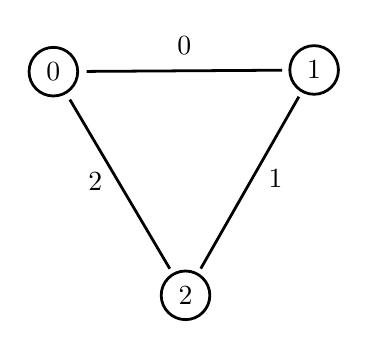
\begin{tikzpicture}[>=latex,line join=bevel,real/.append style={circle, draw=black} ]
  \pgfsetlinewidth{1bp}
%%
\pgfsetcolor{black}
  % Edge: 0 -- 1
  \draw [] (-35.2bp,26.724bp) .. controls (-15.446bp,26.841bp) and (15.392bp,27.043bp)  .. (35.2bp,27.159bp);
  \definecolor{strokecol}{rgb}{0.0,0.0,0.0};
  \pgfsetstrokecolor{strokecol}
  \draw (0bp,35.941bp) node {0};
  % Edge: 2 -- 0
  \draw [] (-5.2199bp,-44.329bp) .. controls (-14.277bp,-29bp) and (-31.973bp,0.95243bp)  .. (-41.211bp,16.588bp);
  \draw (-32.1bp,-12.8705bp) node {2};
  % Edge: 1 -- 2
  \draw [] (41.229bp,17.623bp) .. controls (32.319bp,2.0092bp) and (14.815bp,-28.662bp)  .. (5.9095bp,-44.269bp);
  \draw (32.8bp,-12bp) node {1};
  % Node: 1
\begin{scope}
  \definecolor{strokecol}{rgb}{0.0,0.0,0.0};
  \pgfsetstrokecolor{strokecol}
  \draw (46.722bp,27.249bp) node [real] {1};
\end{scope}
  % Node: 0
\begin{scope}
  \definecolor{strokecol}{rgb}{0.0,0.0,0.0};
  \pgfsetstrokecolor{strokecol}
  \draw (-47.146bp,26.633bp) node [real] {0};
\end{scope}
  % Node: 2
\begin{scope}
  \definecolor{strokecol}{rgb}{0.0,0.0,0.0};
  \pgfsetstrokecolor{strokecol}
  \draw (0.42374bp,-53.881bp) node [real] {2};
\end{scope}
%
\end{tikzpicture}


	\end{center}

\vspace{-0.5cm}
\end{exmp*}

\subsection*{Achieving the canonical generation within Algorithm \ref{algorithm-one_stage}}

\begin{itemize}
	\item At the beginning of each stage the edge $c$ which is being added to $X$ has to satisfy $\iota(c) > \tau(Y)$. Note that as a result the spanning forest $F$ has to be recomputed at the beginning of each stage

	\item Within each stage, after the first edge has been chosen then all the edges $c'$ being added to $X$ have to satisfy $\iota(c') > \tau(Y)$

	\item The path $P$ is chosen on line 18 such that it satisfies the condition of Definition \ref{can}.c.

	\item The choice of edge $c \in E(P) \cap Z^j$, such that it is the edge in $E(P) \cap Z^j$ closest to $T_r$, is embedded in the algorithm by iterating through the edges of $P$ \textit{in order} ("red $\rightarrow$ blue")

\end{itemize}

\clearpage

\begin{algorithm}
	\caption{One canonical stage of stepwise implementation}
	\label{algorithm-can_one_step}
\begin{algorithmic}[1]
	\Require A connected graph $G$, parameters $j,\, k,\, m \in \mathbb{N},\, j < k,\, m \geq 1$ and a~$j$-bond $Y_1 \subseteq E(G)$
	\Ensure A collection of $(j+1)$-bonds as in Algorithm \ref{algorithm-one_stage}), such that each one is in the unique canonical form extending $Y_1$

	\If{$j=1$}
		\State $F \leftarrow$ a $\iota$-minimum spanning forest of $k-1$ trees
		\Else
		\State $F \leftarrow$ a $\iota$-minimum spanning forest of $k-2$ trees, $\lvert F \cap Y_1 \rvert = 1$
	\EndIf

	\ForAll{$d = \{u, v\} \in F \setminus \{e \in E(G) \mid \iota(e) \leq \tau(Y_1) \} $}
		\State \textbf{if} $ \, \nu(v) < \nu(u)$ \textbf{then}  $u,v \leftarrow v, u \,$ \textbf{fi}
		\State \Call{GenStage}{$j, Y_1, X = \{d\}, V_r = \{u\}, V_b = \{v\}, T_r = \{u\}$}
	\EndFor

	\Procedure{GenStage}{$j, Y, X, V_r, V_b, T_r$}
	\State Let $G_1 \subseteq G$ be the conn. component of $G \setminus Y$ containing $X$
	\If{$\lvert Y \cup X \rvert > m - k + j + 1$}
		\State \textbf{return;}
	\EndIf
	\If{there does not exist a connected subgraph \\ \qquad \enspace  $T_b \subseteq (G_1 \setminus V(T_r)) \setminus X$ such that $V_b \subseteq V(T_b)$}
		\State \textbf{return;}
	\EndIf
	\State $P' \leftarrow$ a path $P' \subseteq G_1$ connecting some $r \in V_r$ and $b \in V_b$ \\
	\qquad \quad \,\,\, minimizing $(\lvert E(P) \rvert, \mlen_\lambda(P), \vec{\iota}(P) )$
	\State $P \leftarrow P' \setminus T_r$
	\If{such $P$ does not exist}
		\State \textbf{return} $Y \cup X$ \Comment{$Y \cup X$ is a $j+1$-bond}
	\Else
		\ForAll{$c \in P$}
			\If{$\iota(c) < \tau(Y \cup X)$}
				\State \textbf{continue}
			\EndIf
			\State Let $u$ be the vertex in $c = \{u,v\}$ which is closer to $T_r$
			\State Let $P_u$ be the component of $P - c$ which contains $u$
			\State \Call{GenStage}{$j, Y, X \cup \{c\}, V_r \cup \{u\}, V_b \cup \{v\}, T_r \cup P_u$}
		\EndFor
	\EndIf

	\EndProcedure
\end{algorithmic}
\end{algorithm}

\clearpage


\begin{lem}
	\label{lem:alg_is_canonical}
	Let $G$ be a connected graph. If an implementation of Algorithm \ref{algorithm-one_stage} satisfies the conditions of Definition \ref{can}, namely

	\begin{itemize}
		\item the spanning forest selected at the beginning of each stage (in \textsc{ExtendBond}) is chosen such that it is the unique minimal one with respect to edge weights $\iota$
		\item each path $P$ is chosen such that it lexicographically minimizes the triplet $(\lvert E(P) \rvert, \mlen_\lambda(P), \vec{\iota}(P) )$
	\end{itemize}

	then every generated partition $\mathcal{Z}$ of each $k$-bond $X \subseteq E(G)$ is in its canonical form $can(\mathcal{Z})$.
\end{lem}

\begin{proof}
	Directly from Algorithm \ref{algorithm-can_one_step}.
	\begin{itemize}
		\item The condition \ref{can}.a is satisfied due to line 7.
		\item The condition \ref{can}.b is satisfied by choosing the minimum spanning forest on lines 2, 4 and by the condition on line 26.
		\item The condition \ref{can}.c is satisfied by the choice of $P$ on line 19.
	\end{itemize}
\end{proof}

\noindent The following theorem is a direct consequence of Theorem \ref{thm:stepwise_impl_correctness} and Lemma \ref{lem:every_kbond_has_can}.


% TODO: Is the "\vec X = \mcan(X)" part allowed with the current definition of can(X), where X is a bond?
\begin{thm}
	Let $G$ be a graph, $k \geq 2$, $m \geq 1$ integers. Recursive application of Algorithm \ref{algorithm-can_one_step} generates at least one canonical form $\vec X = \mcan(X)$ of every $k$-bond $X \subseteq E(G)$, $\lvert X \rvert \leq m$.
\end{thm}


The corollary below allows the implementation to slightly differ from the definition of $\mcan()$ without losing correctness. This changes our further use of the term \textit{unique shortest path}.

\begin{cor}
	Algorithm \ref{algorithm-can_one_step} can be modified to always choose the unique shortest path to be a $V(T_r){-}V_b$ path.
\end{cor}

TODO: explanation

\begin{claim}
	\label{forest_sel_claim}
	Algorithm \ref{algorithm-can_one_step} remains correct if in the first step, for both $j = 1$ and $j \leq 2$, it selects $F$ as the minimum spanning forest ${F \subseteq (G \setminus Y)}$ consisting of $k-1$ trees.
\end{claim}

\section{Complete algorithm}

In this section we provide the final version of the circuit-cocircuit algorithm which is used for our practical implementation. Before doing so we introduce several small changes.


\subsection*{Heuristic for the test of hyperplane existence}
Recall that in a given graph $G$ we are avoiding non-minimal cuts $X \subseteq E(G)$ by using a test for the existence of a hyperplane of $G$ in $G \setminus X$. As a helper tool we are using colouring of the graph as described previously.

Previously, we used a basic hyperplane existence test based on performing a graph traversal each time an edge is added to $X$. Now we propose a heuristic which avoids repeated traversal.

\begin{claim}
	Let $G$ be a graph and $X \subseteq E(G)$. Assume there is a blue subgraph interconnecting $V_b$ and perform \textit{check} for a possible disconnection each time some edge $c$ is added to $X$. If this check is positive then a graph traversal is performed and, if possible, a new subgraph interconnecting $V_b$ is found. This \textit{check} can be a heuristic with false positives but no false negatives.
\end{claim}

To implement this technique, the algorithm has a variable for a connected blue subgraph $G_b \subseteq (G \setminus T_r) \setminus X$ such that $V_b \subseteq G_b$. When adding some edge $c$ to $X$ we \textit{check} whether this causes disconnection of $G_b$ with a method which treats $G_b$ as a tree, resulting in a quick test. In case this \textit{check} is positive we attempt to find ("re-create") a new connected subgraph $G_b' \subseteq (G \setminus T_r) \setminus X$ such that $V_b \subseteq V(G_b')$. If $G_b'$ could not be found the algorithm skips further computations using $X \cup \{c\}$. If $G_b'$ was found the algorithm continues its operation with $X \cup \{c\}$ and $G_b := G_b'$.

As suggested the assumption that $G_b$ is a tree may not be correct\footnote{This may happen due to the choice of paths in the "re-creation" procedure and in the \lstinline|shortestPath| procedure} -- in this case the test reported false positive and a new connected blue subgraph $G_b' \subseteq G$ such that $V_b \subseteq V(G_b)$ is found although the previous one might have been connected.

Details on implementing \textit{check} and finding a new ("re-creating") blue subgraph are given in Chapter \ref{ch:practical_impl}.

\subsection*{Aborting \lstinline|GenStage| after losing a hyperplane}

\begin{claim}
	Algorithm \ref{algorithm-can_one_step} may end the execution of a \lstinline|GenStage| call right after adding $c$ to $X$ if it results in $G \setminus X$ having no hyperplane of $G$.
\end{claim}


\clearpage

\begin{algorithm}
	\caption{Canonical stepwise algorithm}
	\label{alg:final}
\begin{algorithmic}[1]
	\Require A graph $G$, $k,m \in \mathbb{N}, m \geq 1$
	\Ensure All $k$-way bonds of $G$ in canonical form and with $\leq m$ edges

	\State \Call{ExtendBond}{$j = 1, Y = \varnothing, V_r = \varnothing, V_b = \varnothing, T_r = \varnothing, G_b = \varnothing$}
	\Procedure{ExtendBond}{$j, Y, V_r, V_b, T_r, G_b$}
	\State $F \leftarrow$ $\iota$-minimum spanning forest $F \subseteq (G \setminus Y )$ on $k-1$ trees
	\ForAll{$d = \{u, v\} \in F \setminus \{e \in E(G) \mid \iota(e) < \tau(Y) \}$}
		\State \textbf{if} $ \, \nu(v) < \nu(u)$ \textbf{then}  $u,v \leftarrow v, u \,$ \textbf{fi}
		\State \Call{GenStage}{$j, Y, \{d\}, \{u\}, \{v\}, \{u\}, \{v\}$}
	\EndFor
	\EndProcedure

	\Procedure{GenStage}{$j, Y, X, V_r, V_b, T_r, G_b$}

	\State Let $G_1 \subseteq G$ be the conn. component of $G \setminus Y$ containing $X$

	\If{$\lvert Y \cup X \rvert > m - k + j + 1$}
		\State \textbf{return;}
	\EndIf

	\State $P \leftarrow$ a path $P \subseteq G_1$ connecting some $r \in V(T_r)$ and $b \in V_b$ \\
	\qquad \quad \,\,\, minimizing $(\lvert E(P) \rvert, \mlen_\lambda(P), \vec{\iota}(P) )$

	\If{such $P$ does not exist}
		\State \textbf{if} $j = k - 1$ \textbf{then} \textbf{return} $Y \cup X$ \Comment{$X$ is a $k$-bond}
		\State \textbf{else} \Call{ExtendBond}{$j + 1, Y \cup X, \varnothing, \varnothing, \varnothing, \varnothing$} \textbf{fi}

	\Else
		\ForAll{$c = \{u, v\} \in P$}
			\State Let $u$ be the vertex in $\{u,v\}$ which is closer to $T_r$
			\State Let $P_u$ be the component of $P - c$ which contains $u$
			\State Let $P_v$ be the component of $P - c$ which contains $v$
			\If{$G_b \sm \{c\}$ is disconnected}
				\State $G_b \leftarrow$ a new subgraph interconnecting $V_b$
				\State \textbf{if} such $G_b$ cannot be found \textbf{then} \textbf{return;}
			\EndIf
			\If{$\iota(c) < \tau(Y \cup X)$}
				\State \textbf{continue}
			\EndIf
			\State \textsc{GenStage}($j, Y, X \cup \{c\}, V_r \cup \{u\}, V_b \cup \{v\},$ \\
			\hskip 116.8pt $T_r \cup P_u, G_b \cup P_v$)
		\EndFor
	\EndIf

	\EndProcedure
\end{algorithmic}
\end{algorithm}


\chapter{Practical implementation}
\label{ch:practical_impl}

The source code of our implementation is stored in a git repository on GitHub\footnote{\url{www.github.com}} available online at \url{https://github.com/OndrejSlamecka/mincuts}. This repository also contains tools related to working with the output of the main program called \lstinline|mincuts| and measuring of various parameters further described in Chapter 6. Short documentation can be found in \lstinline|readme.md|. The source code is available under MIT license \footnote{\url{http://opensource.org/licenses/MIT}} enclosed within the repository.

\section{Choice of tools}

To implement the algorithm we are using the C++ programming language, which is a popular language with very fast execution of the resulting programs (on general computing problems). We are using the C++11 standard and the source code was successfully compiled with \lstinline|gcc| version 4.8.2.

To avoid reinventing the wheel with basic data structures (e.g. graph, disjoint sets) we are using a small part of OGDF -- Open Graph Drawing Framework. This small part has no graph drawing related burden and thus does not interfere with our goal. Also this dependency could be easily replaced by own implementation.

\section{Choice of $\lambda$}
\label{sec:choice_of_lambda}

Recall $\lambda$ is an arbitrary map $E(G) \rightarrow \mathbb{N}$ used in the algorithm to select the unique canonical path between some vertex of $V(T_r)$ and some of $V_b$. We will also describe the use of this map in self-testing procedures. The choice of $\lambda$ is done before starting the circuit-\linebreak{}cocircuit algorithm.

In an ideal setting $\lambda$ would be chosen such that $\lambda(e) := 2^{\iota(e)}$. With this choice no two paths $P_1, P_2 \subseteq G$ could have $\mlen_{\lambda}(P_1) = \mlen_{\lambda}(P_2)$. But this choice is not feasible for any but small graphs due to the limits on the size of integer variables.

Instead we implemented a trivial approach which yields practically goods results (measured in Chapter \ref{chapter_evaluation}). For each $e \in E(G)$ we set $\lambda(e) := r_e$, where $r_e$ is a number chosen from the range $[0, \, { {m}\over{|V| - k + 1} } )$ with uniform probability. Here $m$ stands for the highest value a variable of type \lstinline|uint64_t| \footnote{\lstinline|uint64_t| is defined in header file \lstinline|cstdint|} can hold and $k$ is the input parameter of the algorithm specifying the multiplicity of the cuts (it is the $k$ in $k$-bonds).

The upper bound on $r_e$ is chosen as such because a type-C circuit is of length at most $\lvert V \rvert - k + 2$ -- we have to avoid exceeding the maximum value of an \lstinline|uint64_t| variable when computing $\mlen_\lambda$.

Our implementation uses various tools from the C++11 standard library: random engine \lstinline|default_random_engine|, random number distribution \lstinline|uniform_int_distribution| and \lstinline|random_device| to seed the \linebreak random engine.


\section{Choice of forest in \lstinline|ExtendBond|}

Let $G$ be a graph, $k$ the given multiplicity of the resulting cuts and $Y$ a $j$-bond such that $j < k$. In our implementation we are using Kruskal's algorithm to find the $\iota$-minimum spanning forest $F \subseteq G$ with the following modifications:

\begin{itemize}
	\item we avoid adding edges of $Y$ to $F$ (confer Claim \ref{forest_sel_claim}),
	\item we stop generating $F$ when $\lvert E(F) \rvert = |V(G)| - (k - 1)$, because this is the number of edges a forest of $k - 1$ trees has.
\end{itemize}

With the canonical generation the algorithm does not start generation from those edges $e$ of $F$ which satisfy $\iota(e) \leq \tau(Y)$ (confer Definition \ref{def:tau}). Such comparison is possible by maintaining a variable we call \lstinline|lastBondFirstEdge| together with the variable $X$ (confer Algorithm \ref{alg:final}). In this variable we are storing the edge $c_{s(j)+1}$, where $j$ is the largest index such that $c_{s(j)+1}$ has been added to $X$. From its definition the variable is updated at the beginning of each stage.

\section{Graph colouring}
\label{sec:colouring}

To hold the colouring of vertices and edges in the memory we use a single map \textit{colouring} : (\textit{Vertex} or \textit{Edge}) $\rightarrow \{$\textit{red}, \textit{blue}, \textit{black}$\}$, where \textit{black} serves no special purpose but marking that an edge hasn't been coloured red or blue.

Object \lstinline|colouring|, an instance of class $GraphColouring$ defined in the C++ code to represent the \textit{colouring} from above, stores the colouring internaly as maps from \textit{node} and \textit{edge} types to enumerated type \textit{Colour}. The class also maintains a list of all red vertices and a counter of blue vertices to achieve faster access to this information.

For vertices the class offers \lstinline|set(vertex, colour)| as a setter and an overloaded array access operator as a getter. For edges overloaded array operator is used for both changing and reading the information about edge colour. An example of changing the colour of edge $e$~would be \lstinline|colouring[e] = Colour::BLUE|.

When implementing the colouring it was necessary to allow for

\begin{enumerate}
	\item fast computation of the unique shortest $V(T_r){-}V_b$ path,
	\item quickly answering whether $G \setminus X$ contains a hyperplane.
\end{enumerate}

Before we continue to specific implementation details of those two tasks let us note:

\begin{itemize}
	\item it will turn out that in $T_b$ we do not need to recognize, and thus do not need to colour, other vertices as blue than those in $V_b$,

	\item when adding each edge $c$ from the path (between $V(T_r)$ and $V_b$) to $X$ we would have to colour blue the part of the path from $c$ to the blue tree. To avoid repetition we instead colour the whole path blue right after finding the path.
\end{itemize}


\section{Graph colouring memory management}

When considering the level $i$ of recursion of the algorithm within the $j$-th stage, one notices that the colouring of the graph on levels~${>i}$ must not affect the colouring on the level $i$. A simple solution to this problem would be to copy the whole part of memory containing the colouring when entering a new level of recursion. However such copying greatly reduces the speed of the program. For example when computing $4$-bonds with up to four edges of the road network of the Zlín Region, the original program computes the bonds faster than a modified one (with copying of the colouring) by 26\%.

So in order to improve the efficiency of our implementation we want to avoid copying of the object containing the colouring as much as possible. The program does this by passing \lstinline|colouring| by reference, recording every step of colouring done on the level $i + 1$ of recursion and at the end of this level reverting the steps to leave the colouring as it was before entering it. Note that with each \lstinline|ExtendBond| call we need to start the whole colouring again so here we actually create a new object of class \lstinline|GraphColouring|.

In each call of \lstinline|GenStage| after successfully finding the path $P$ we start by colouring the path blue. Before doing so we have to record which edges of the path are blue (to correctly restore the state of colouring later). In the case of disconnecting the blue subgraph $G_b$ we also need to record the edges of this old, disconnected graph and then record the edges of the new blue tree.

At the end of \lstinline|GenStage| execution (all the edges of $P$ were considered or there is no hyperplane) we call the \lstinline|revertColouring| procedure to set the colouring back to the state in which it was before entering this \lstinline|GenStage|. First, $G_b$ disconnection occurred, then we colour black the edges of the newly created blue tree and the edges of the old blue tree (recoloured black in this stage) are coloured blue. Then we colour both edges and vertices of the path black. We might have coloured black some blue vertex of $X$ during the stage so we colour all non-red vertices of $X$ blue (note that we could not have lost a red vertex). Then we colour blue all the edges which are in the path but were blue before this stage.

\clearpage

\section{Finding the (unique) shortest path}

In this section we give details about implementing the \lstinline|shortestPath| procedure. Let $G, Y, X, T_r, V_b$ be as in Algorithm \ref{alg:final}.

First, we look into the situation of Algorithm \ref{algorithm-one_stage}, that is without canonical generation. The search procedure has to find a $V(T_r){-}V_b$ path. Since our implementation actually colours blue only vertices in $V_b$ we can translate the problem to finding the shortest path between some red vertex and some blue vertex. To solve this problem we are using a slight modification of the breadth-first search algorithm. In this modification the algorithm starts the search not from a single vertex but from all red vertices\footnote{Thus it does not necessarilly generate a BFS tree, it is a BFS forest} and then continues searching through $G \setminus (X \cup Y \cup E(T_r))$ until a blue vertex is found. The algorithm then returns the found path.

Note that this modifiaction of BFS creates a BFS forest rather than a BFS tree. By the distance of a vertex $n$ we mean the distance of the shortest path from $n$ to some of the starting vertices.

Now we investigate the choice of the unique shortest path. Recall that the unique shortest path is the path $P$ which lexicographically minimizes $(\lvert P \rvert, len_\lambda(P), (\iota(e_1), ...,\iota(e_{\lvert P \rvert}))$. The algorithm chooses $\lambda$ \linebreak during initialization, see Section \ref{sec:choice_of_lambda}.

For each vertex $v$ we define the \textit{$\lambda$ distance}, denoted $d_\lambda(v)$, such that $d_\lambda(v) = \mlen_\lambda(Q)$, where $Q$ is the shortest path\footnote{Without this restriction we would need for example Dijkstra's algorithm} from some of the starting vertices. $d_\lambda(s) = 0$ for each starting vertex $s$.

We further modify the BFS-like algorithm from above to compute the $\lambda$ distance. The algorithm recognizes two cases; say it has encountered a vertex $v$:

\begin{itemize}
	\item if $v$ was just discovered from $u$ through edge $e$ -- then the algorithm sets $d_\lambda(v) := d_\lambda(u) + \lambda(e)$,

	\item if $v$ was discovered previously from $u$, but now the algorithm explores an edge $f = \{u', v\}$, such that $u'$ is in the same distance as $u$ -- then the algorithm sets $d_\lambda(v) := d_\lambda(u') + \lambda(f)$ and updates the BFS forest (to mark $u'$ to be the predecessor of $v$) only if $d_\lambda(v)$ would decrease.

\end{itemize}

Since the algorithm updates $d_\lambda$ only in vertices at the maximum currently discovered distance and since it is a modification of BFS\footnote{Vertices are discovered in the order determined by their distance from the start}, one can use an easy induction on the maximum discovered distance to prove the correctness of computing $d_\lambda$.

	It is important that we cannot end the search right away when some blue vertex $n$ is discovered. The algorithm has to empty the queue it uses (without further exploration of more distant vertices) since there may be a blue vertex $m$ in the same distance as $n$. This finishes minimizing $(\lvert P \rvert, \mlen_\lambda(P))$.

	However there may still be two paths $P_1$ and $P_2$ which are equal when comparing $(\lvert P_1 \rvert, \mlen_\lambda(P_1))$ and $(\lvert P_2 \rvert, \mlen_\lambda(P_2))$. We choose the one which minimizes $\vec{\iota}(P) = (\iota(e_1), \iota(e_2),\ldots, \iota(e_{\lvert P \rvert}))$ with an easy comparison. This finishes the canonical choice of the unique shortest path $P$ between some vertex of $V(T_r)$ and some vertex of $V_b$.

\section{Hyperplane detection}

We will give details on implementing the heuristic which was used in Chapter \ref{ch:canonical}. Let $G, X, G_b$ be as in Algorithm \ref{alg:final}.

\subsection*{Testing possible disconnection of $G_b$}

To answer the question whether adding a new edge $c = \{u,v\}$ to $X$ causes a disconnection of $G_b$ we would generally need graph traversal algorithms again. If $G_b$ was a tree and we did not colour the shortest path blue right after finding it (confer Section \ref{sec:colouring}) then the question is equivalent to $c$ being blue (by the definition of tree). The problem is that this assumptions are not fulfilled in our setting:

\begin{enumerate}
	\item $G_b$ may not be a tree, this may result in false positives,
	\item $c$ is always blue since we colour blue the path found at the beginning of \lstinline|GenStage| call.
\end{enumerate}

As described previously our algorithm handles false positives sufficiently well, so we can assume $G_b$ is a tree. The second problem can be avoided by investigating the colours of the edges (other than $c$) incident to $u$ and $v$. Two situations can arise now:

\begin{enumerate}
	\item the edge $c$ would be in the blue tree even if we didn't colour the path blue first
	\item the edge $c$ is not in the blue tree, but $u$ or $v$ are
\end{enumerate}

In both cases note that $u \not \in V_b(X)$ from the definition of our path.

In the first case $c$ may be connecting a leaf in $V_b$ to the rest of the graph. $u$ cannot be this leaf. If edge $c$ was connecting $v$ to the rest of $T_b$ then some edge incident to $u$ must be blue.

In the second case, if only $v$ is blue then no disconnection happens, since $v$ is going to be coloured blue. If $u$ is blue, then some edge incident to $u$ (besides $c$) must be blue.

In conclusion, colouring $u$ red, $v$ blue and $c$ black disconnects the blue tree, if and only if, $u$ is incident to a blue edge different from $c$.

\subsection*{Finding a new blue subgraph interconnecting $V_b$}

In an attempt to find a new blue subgraph $G_b'$ interconnecting $V_b$ we first colour the old $G_b$ black and then find $G_b'$ if possible. Finding $G_b'$ is done by breadth-first searching $G$ starting from some blue vertex of $X$ and counting the blue vertices which were found. Each time a blue vertex is found we colour the path from this vertex to the starting one blue, increase the counter marking how many of blue vertices we found and if this counter is equal to $\lvert V_b \rvert$ then we succeeded. If the search ends without reaching this equality the re-creation of blue subgraph has failed.

\section{Testing correctness}

Although we have given a proof of correctness of the algorithm in chapters \ref{ch:algorithm} and \ref{ch:canonical}, we also employ several approaches to discover possible errors in transcription of the algorithm into C++ code. The first approach is testing with mechanisms built directly into the implementation.

The other two approaches are systematic and randomized testing of the algorithm against a combinatorial "brute-force" algorithm. This algorithm simply enumerates all the possible combinations of less than $m$ edges and evaluates whether or not they form a $k$-bond by using the \lstinline|isMinCut| function\footnote{Defined in \lstinline|src/helpers.cpp|}.

We implement the systematic and randomized tests in a program called \lstinline|tester|. This program calls repeatedly procedure \textit{check} with arguments depending on the source of graphs (random generation or standard input).

The \textit{check} used above works as follows: For given $G$, $m$, $k$ the procedure calls function \lstinline|bruteforceGraphBonds| and the \textit{circuit-cocircuit} algorithm implementation. Then it computes the symmetric difference of the results and returns \textit{true} if and only if the symmetric difference is empty.

To speed up the testing process \lstinline|tester| implements a simple parallelization. Each thread requests graphs from a shared "storage" and performs the check. In the randomized tester we avoid using locks -- the result is a faster execution at the cost of occasionally garbled output. These two effects are notable only when generating small graphs.


\subsection*{Selftesting procedures}

The algorithm contains methods to reveal errors due to graph traversal order (and thus choice of paths and the choice of a new blue tree interconnecting $V_b$).

One is directly embedded in the choice of the unique shortest path. Recall the unique shortest path $P$ is chosen such that it minimizes the triplet $(\lvert P \rvert, len_\lambda(P), (\iota(e_1), ...,\iota(e_{\lvert P \rvert}))$. The map $\lambda$ is selected at random with each run of the algorithm to randomize the selection of the unique shortest path. Repeated tests have shown that this method is effective -- we intentionally changed the implementation to be incorrect in several ways and then observed different output with each run of the program.

Second method of testing the algorithm right within the implementation is to change the bijection $\iota : edge \rightarrow \mathbb{N}$ such that if $G$ is a graph and the function $\iota$ is given with this graph then $\forall e \in E(G)$ we set $\iota(e) := m - \iota(e)$ where $m = max \{ \iota(e) \mid e \in E(G) \}$. This makes the algorithm choose the forest $F$ (both as a basis and as a $k$-way circuit) as different as possible from the forest which would be chosen with the original $\iota$. Effectiveness of this method was successfully tested as above.

\subsection*{Using systematic graph generator}

To prove the correctness of the implementation for graphs on $\leq 32$ vertices one could use a systematical graph generator \lstinline|geng| from package \lstinline|nauty| \cite{mckay_isom}. Program \lstinline|tester| reads graphs from the standard input and checks the algorithm against them. The graphs are expected to be in graph6 format, which is the same nauty's \lstinline|geng| produces. An easier to use tool called \lstinline|geng_tester.sh| is given in the folder \lstinline|tools|, this tool calls the graph generator \lstinline|geng| and redirects the output to our \lstinline|tester|.

The program has been successfully tested on all 261080 mutually non-isomorphic connected graphs on nine vertices when finding $2,3,4,5$-bonds with up to $5$ edges.

\subsection*{Randomly generated graphs}

The systematical approach above is good if we have vast computational resources. However this is often not the case (given the number of graph isomorphism classes) and if we aim to demonstrate an error in the implementation then picking random graphs might reveal mistakes earlier.

We are using the \lstinline|randomSimpleGraph| function from OGDF to generate random graphs on a given number of vertices and edges. These graphs are not guaranteed to be connected -- we make them connected by adding additional edges between the trees of the depth-first search traversal forest. As a result the requested number of edges is exceeded, but a slight variation does not interfere with the purpose this tester was built for.

A different approaches to generate random graphs were explored but they were notably slower. Namely generating a random tree (using \lstinline|randomTree| from OGDF) and then adding the remaining edges at random was about two times slower. If this tree was to be generated with uniform probability (for example with Wilson's UST algorithm) it would again slow the testing down, this time very significantly.


\chapter{Evaluation}
\label{chapter_evaluation}

\section{Running time}

For the running time evaluation we used a computer with 16 GB RAM and The Intel(R) Core(TM) i7-3770 CPU @ 3.40GHz. The source code was compiled with \lstinline|gcc| 4.8.2 and the \lstinline|-O3| flag to enable compiler optimizations.

First we give an overview of running time on different graphs with variable choice of parameters $k$ (as in $k$-bond) and $m$ (maximum size of a bond). These running times were measured using the GNU \lstinline|time| utility. Time spent interacting with the operating system was not included in the measurement.

Then we show how much time is spent generating the $k$-bonds from edge $e \in F$, where $F$ is the spanning forest chosen in the first steps of the algorithm. Here $\mtime(e)$ is the number of milliseconds the program runs in the branch of computation starting with $X = \{e\}$ and $\mbonds(e)$ is the number of bonds it generated, $Q_p$ is $p$-th quantile of the time attribute of the data set. Based on the following $\chi$ function, we define $\mathcal{P}(x,y) = \{ e \in F : \chi(x,y,e) = 1 \}$ and $\#Q_x, Q_y = \lvert \mathcal{P}(x,y) \rvert$.

\[
	\chi(x, y, e) \stackrel{\text{def}}{=}
	\begin{cases}
		\hfill 1  \hfill & \text{\textbf{if} $Q_x < \mtime(e) \leq Q_y$ \break \textbf{or} $x=0 \wedge \mtime(e) = Q_x$,} \\
		\hfill 0  \hfill & \text{otherwise} \\
	\end{cases}
\]

\[
	\Sigma Q_x, Q_y \stackrel{\text{def}}{=} \sum_{e \in \mathcal{P}(x,y)} \mbonds(e)
\]

To measure elapsed $\mtime$ we are using \lstinline|process_user_cpu_clock| from the \lstinline|boost::chrono| \thinspace C++ library. This clock reports CPU time spent by the current process in the user space (i.e.\ the time interacting with the operating system was not included).


\clearpage

%%% Runtime Zlin

\subsection*{Zlín Region (723 vertices, 974 edges)}

In Figure \ref{fig:zlin_rtm} we can see how the time taken depends on the number of bonds produced when generating a family of bonds (all bonds in the family having a common first edge). Table \ref{table:zlin-rtm-stat} shows that the quarter of the longest taking computations generate the majority of bonds.


\begin{table}[H]
	\caption{Running time in seconds for different choices of $k$ (rows) and $m$ (columns)}
	\centering
	\begin{tabular}{c|rrrrrrrr}

\toprule

	&         2 &         3 &         4 &         5 &         6 &         7 &		8 	\\ \midrule
 2	&      0.03 &      0.10 &      0.40 &      1.69 &      8.47 &     42.60 &	210.34	\\
\evenrowcolor
 3	&      0.57 &      2.77 &     12.50 &     53.38 &    223.15 &    986.02 &	4603.89	\\
 4	&           &     29.49 &    197.92 &   1018.22 &   4771.04 &  21269.76 &	-		\\
\evenrowcolor
 5	&           &           &   1155.52 &   9884.54 &  56847.00 &	-	   & 	-		\\

	\end{tabular}
\end{table}

\vspace{-0.5cm}
\begin{figure}[H]
	\caption{Each point represents the process of generating bonds starting with an edge of the $k$-way basis, here $k = 4$ and $m = 4$}
	\label{fig:zlin_rtm}

	\centering
	\begin{gnuplot}[terminal=epslatex, terminaloptions=color]
		unset key

		set style line 1 lc rgb 'black' pt 2   # square
		set style line 12 lc rgb'#808080' lt 0 lw 1
		set grid back ls 12

		set xtics nomirror rotate by -45
		set format x '%.0s %c'

		set xlabel "Number of generated $k$-bonds"
		set ylabel "Time to taken (ms)"
		plot "data/rtm/rtm-zlin-4-4-d1.dat" using 3:2 with points ls 1
	\end{gnuplot}
\end{figure}

\vspace{-1cm}

\begin{table}[H]
	\caption{Statistics of the data set used in Figure \ref{fig:zlin_rtm}. Computations with $\mtime(e) = \mbonds(e) = 0$ excluded}
	\label{table:zlin-rtm-stat}
	\centering
	\begin{tabular}{rr||rr|r|r}

\toprule
$p_1$	&	$p_2$		& $Q_{p_1}$	& $Q_{p_2}$	& $ \#Q_{p_1},Q_{p_2} $ & $ \Sigma Q_{p_1},Q_{p_2} $ \\ \midrule

0	&	0.25	& 0	&	110	& 72	& 44753 \\
\evenrowcolor
0.25	&	0.5	& 110	&	340	& 70	& 262593 \\
0.5	&	0.75	& 340	&	1175	& 70	& 678110 \\
\evenrowcolor
0.75	&	1	& 1175	&	9730	& 71	& 2858919 \\

	\end{tabular}
\end{table}


%%% Runtime Olomouc

\subsection*{Olomouc Region (1454 vertices, 2066 edges)}

In the Olomouc Region a bigger part of the resulting bonds is generated by the quarter of the edges with the lowest $\mtime(e)$ than in Zlín Region. This can be seen in Figure \ref{fig:olomouc_rtm} and Table \ref{table:olomouc-rtm-stat}.

\begin{figure}[H]
	\caption{Each point represents the process of generating bonds starting with an edge of the $k$-way basis, here $k = 3$ and $m = 7$}
	\label{fig:olomouc_rtm}

	\centering
	\begin{gnuplot}[terminal=epslatex, terminaloptions=color]
		unset key

		set style line 1 lc rgb 'black' pt 2   # square
		set style line 12 lc rgb'#808080' lt 0 lw 1
		set grid back ls 12

		set xtics nomirror rotate by -45
		set format x '%.0s %c'

		set xlabel "Number of generated $k$-bonds"
		set ylabel "Time to taken (ms)"
		plot "data/rtm/rtm-olomouc-7-3-d1.dat" using 3:2 with points ls 1
	\end{gnuplot}
\end{figure}

For clarity Figure \ref{fig:olomouc_rtm_under30k_ms} displays the same data as Figure \ref{fig:olomouc_rtm} but without the very few records with long time and a great number of bonds produced. We see that the ratio of time taken and number of bonds generated is higher than desirable in some cases.

\begin{figure}[H]
	\caption{Data from Figure \ref{fig:olomouc_rtm} but only records with $\mtime < 30000$ are displayed}
	\label{fig:olomouc_rtm_under30k_ms}

	\centering
	\begin{gnuplot}[terminal=epslatex, terminaloptions=color]
		unset key

		set style line 1 lc rgb 'black' pt 2   # square
		set style line 12 lc rgb'#808080' lt 0 lw 1
		set grid back ls 12

		set xtics nomirror rotate by -45
		set format x '%.0s %c'

		set xlabel "Number of generated $k$-bonds"
		set ylabel "Time to taken (ms)"
		plot "data/rtm/rtm-olomouc-7-3-d1-under30k-ms.dat" using 3:2 with points ls 1
	\end{gnuplot}
\end{figure}

\vspace{-1cm}

\begin{table}[H]
	\caption{Running time in seconds for different choices of $k$ (rows) and $m$ (columns)}
	\centering
	\begin{tabular}{c|rrrrrrrr}

\toprule

        &         1 &         2 &         3 &         4 &         5 &         6 &      7 &      8 \\
\midrule
     2  &      0.02 &      0.07 &      0.30 &      1.28 &      5.15 &     16.16 &     69 &    305 \\
\evenrowcolor
     3  &           &      3.00 &     10.38 &     60.88 &    235.40 &    921.45 &   3482 &  13342 \\
     4  &           &           &    158.29 &    781.43 &   6008.40 &        -  &      - &      - \\
\evenrowcolor
     5  &           &           &           &   6205.22 &  43242.26 &        -  &      - &      - \\



	\end{tabular}
\end{table}


\begin{table}[H]
	\caption{Statistics of the data set used in Figure \ref{fig:olomouc_rtm}. Table excludes computations with $\mtime(e) = \mbonds(e) = 0$}
	\label{table:olomouc-rtm-stat}
	\centering
	\begin{tabular}{rr||rr|r|r}

\toprule
$p_1$	&	$p_2$		& $Q_{p_1}$	& $Q_{p_2}$	& $ \#Q_{p_1},Q_{p_2} $ & $ \Sigma Q_{p_1},Q_{p_2} $ \\ \midrule

0	&	0.25	& 0	&	515	& 358	& 639245 \\
\evenrowcolor
0.25	&	0.5	& 515	&	1290	& 361	& 2257757 \\
0.5	&	0.75	& 1290	&	2980	& 354	& 4128353 \\
\evenrowcolor
0.75	&	1	& 2980	&	104450	& 358	& 12456337 \\
	\end{tabular}
\end{table}



%%% Runtime Stredocesky

\subsection*{Central Bohemian Region (4114 vertices, 5964 edges)}

Measurements with the road network of the Central Bohemian (Středočeský) Region have similar results as those with the Olomouc Region road network. In figures \ref{fig:stredocesky_rtm} and \ref{fig:stredocesky_rtm_4_3} each point represents the process of generating bonds starting with an edge of the $k$-way basis. Figure \ref{fig:stredocesky_rtm} shows an increased number of comparatively slower computations, however this is not significant for greater $m$ as can be seen in \ref{fig:stredocesky_rtm_4_3}.


\begin{table}[H]
	\caption{Statistics of the data set used in Figure \ref{fig:stredocesky_rtm}. Computations with $\mtime(e) = \mbonds(e) = 0$ excluded}
	\label{table:stredocesky-rtm-stat}
	\centering
	\begin{tabular}{rr||rr|r|r}

\toprule
$p_1$	&	$p_2$		& $Q_{p_1}$	& $Q_{p_2}$	& $ \#Q_{p_1},Q_{p_2} $ & $ \Sigma Q_{p_1},Q_{p_2} $ \\ \midrule

0	&	0.25	& 0	&	60	& 240	& 20252 \\
\evenrowcolor
0.25	&	0.5	& 60	&	120	& 216	& 54499 \\
0.5	&	0.75	& 120	&	230	& 209	& 85212 \\
\evenrowcolor
0.75	&	1	& 230	&	560	& 218	& 152298 \\


	\end{tabular}
\end{table}


\begin{table}[H]
	\caption{Running time in seconds for different choices of $k$ (rows) and $m$ (columns)}
	\label{fig:stredocesky_kmvar}
	\centering
	\begin{tabular}{c|rrrrrrrr}

\toprule
        &         1 &         2 &         3 &         4 &         5 &      6 &         7 &         8 \\
\midrule
     2  &      0.24 &      0.72 &      3.85 &     12.71 &     37.85 &    140 &    599 &   2687 \\
\evenrowcolor
     3  &           &     47.32 &    175.76 &   1156.88 &   4480.29 &  18366 &           &           \\

	\end{tabular}
\end{table}


\begin{figure}[H]
	\caption{$k = 3$ and $m = 3$}
	\label{fig:stredocesky_rtm}

	\centering
	\begin{gnuplot}[terminal=epslatex, terminaloptions=color]
		unset key

		set style line 1 lc rgb 'black' pt 2   # square
		set style line 12 lc rgb'#808080' lt 0 lw 1
		set grid back ls 12

		set xtics nomirror rotate by -45
		set format x '%.0s %c'

		set xlabel "Number of generated $k$-bonds"
		set ylabel "Time taken (ms)"
		plot "data/rtm/rtm-stredocesky-3-3-d1.dat" using 3:2 with points ls 1
	\end{gnuplot}
\end{figure}

\vspace{-1cm}

\begin{figure}[H]
	\caption{$k = 3$, $m = 4$}
	\label{fig:stredocesky_rtm_4_3}

	\centering
	\begin{gnuplot}[terminal=epslatex, terminaloptions=color]
		unset key

		set style line 1 lc rgb 'black' pt 2   # square
		set style line 12 lc rgb'#808080' lt 0 lw 1
		set grid back ls 12

		set xtics nomirror rotate by -45
		set format x '%.0s %c'

		set xlabel "Number of generated $k$-bonds"
		set ylabel "Time taken (ms)"
		plot "data/rtm/rtm-stredocesky-4-3-d1.dat" using 3:2 with points ls 1
	\end{gnuplot}
\vspace{-1cm}
\end{figure}

\subsection*{Running time according to graph density}

We show how the number of edges of the given graph affects the time taken generating the bonds. However the figures also show that the number of bonds of given size quickly decreases in denser graphs. The running time decreases too becaus finding the unique shortest path is quick in a dense graph.


\begin{figure}[H]
	\caption{Graphs on 25 vertices, $k = 4$ and $m = 15$}
	\label{fig:density_times}

	\centering
	\begin{gnuplot}[terminal=epslatex, terminaloptions=color]
		unset key

		set style line 1 lc rgb 'black' pt 2   # square
		set style line 12 lc rgb'#808080' lt 0 lw 1
		set grid back ls 12

		set xtics nomirror rotate by -45
		set format x '%.0s %c'

		set ylabel "Time taken (ms)"
		set xlabel "The number of edges in the graph"
		plot "data/density/density-15-4.dat" using 1:2 with points ls 1
	\end{gnuplot}
\end{figure}


\begin{figure}[H]
	\caption{Number of generated bonds (the same data set as in \ref{fig:density_times})}
	\label{fig:density_bonds}

	\centering
	\begin{gnuplot}[terminal=epslatex, terminaloptions=color]
		unset key

		set style line 1 lc rgb 'black' pt 2   # square
		set style line 12 lc rgb'#808080' lt 0 lw 1
		set grid back ls 12

		set xtics nomirror rotate by -45
		set format x '%.0s %c'

		set ylabel "Number of generated bonds"
		set xlabel "The number of edges in the graph"
		plot "data/density/density-15-4.dat" using 1:3 with points ls 1
	\end{gnuplot}
\vspace{-1cm}
\end{figure}

%%%%%%%%%% EFFECTS OF CANONICAL

\section{Acceleration with canonical generation}

We compare the number of generated bonds (including more permutations of the same bond, see section below) with and without canonical generation. Canonical generation was disabled by removing all conditions (introduced in Chapter \ref{ch:canonical}) which resulted in pruning of the search space.

\subsection*{Zlín Region}

\begin{table}[H]
	\caption{How many times is the canonical generation faster for given $k$ (rows) and $m$ (columns)}
	\centering
	\begin{tabular}{c|rrrrrrrr}

\toprule

         &         2 &         3 &         4 &         5 &         6 &         7 \\
\midrule
      2  &        1  &         2 &      2.45 &      3.60 &       4.3 &      1.34 \\
\evenrowcolor
      3  &      3.28 &      3.51 &      6.05 &      8.83 &     12.11 &     14.90 \\
      4  &           &       8.4 &     11.32 &     15.73 &         - &         - \\

	\end{tabular}
\end{table}

\begin{table}[H]
	\caption{How much less ordered bonds does the canonical generation produce for given $k$ (rows) and $m$ (columns)}
	\centering
	\begin{tabular}{c|rrrrrrrr}

\toprule

        &         2 &         3 &         4 &         5 &         6 &         7 \\ \midrule
     2  &      1.43 &      1.97 &      2.67 &      3.52 &      4.42 &      1.15 \\
\evenrowcolor
     3  &      2.00 &      3.08 &      4.27 &      5.99 &      7.94 &     10.09 \\
     4  &           &      6.00 &      9.50 &     13.38 &         - &         - \\


	\end{tabular}
\end{table}


\subsection*{Olomouc Region}


\begin{table}[H]
	\caption{How many times is the canonical generation faster for given $k$ (rows) and $m$ (columns)}
	\centering
	\begin{tabular}{c|rrrrrrrr}

\toprule

   &         2 &         3 &         4 &         5 &         6 &     7 &     8 \\ \midrule
2  &      1.14 &      1.93 &      1.91 &      2.18 &      4.30 &  5.06 &  5.57 \\
\evenrowcolor
3  &      1.97 &      3.47 &      4.49 &      6.69 &      8.31 &     - &     - \\
4  &           &      5.96 &     10.16 &     15.53 &         - &     - &     - \\

	\end{tabular}
\end{table}

\begin{table}[H]
	\caption{How much less ordered bonds does the canonical generation produce for given $k$ (rows) and $m$ (columns)}
	\centering
	\begin{tabular}{c|rrrrrrrr}

\toprule

   &      2 &         3 &         4 &         5 &         6 &         7 &         8 \\ \midrule
2  &   1.32 &      1.93 &      2.53 &      3.26 &      4.04 &      4.78 &      5.51 \\
\evenrowcolor
3  &   2.00 &      2.84 &      4.03 &      5.50 &      7.41 &         - &         - \\
4  &        &      6.00 &      8.79 &     12.37 &        -  &         - &         - \\



	\end{tabular}
\end{table}

%%% Failed to canonize:


\section*{Generated non-canonical permutations}

If we consider canonicity with respect to each bond, not bond and its certain partition as in the definition of $\mcan()$, our algorithm still generates more permutations of the same bond. Due to its complexity and (as demonstrated below) little impact on the result, the algorithm does not perform an explicit isomorphism test for each generated bond. We show an example and document how much is the result non-canonical.

\begin{figure}[H]
	\caption{Let $k = 3$, $m = 3$. In stage 1 the algorithm generates bonds 0,1 and 0,2. In stage 2 bond 0,1 is extended to 0,1,2 and bond 0,2 is extended to 0,2,1. }
\begin{center}
	% 
% dot2tex --autosize tmp/graph9.tmp --prog neato --figonly
%

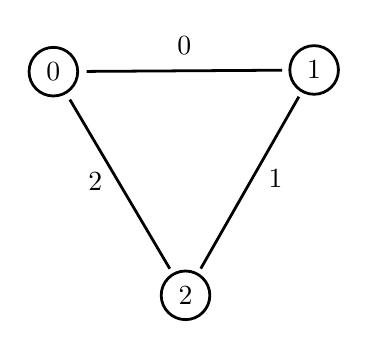
\begin{tikzpicture}[>=latex,line join=bevel,real/.append style={circle, draw=black} ]
  \pgfsetlinewidth{1bp}
%%
\pgfsetcolor{black}
  % Edge: 0 -- 1
  \draw [] (-35.2bp,26.724bp) .. controls (-15.446bp,26.841bp) and (15.392bp,27.043bp)  .. (35.2bp,27.159bp);
  \definecolor{strokecol}{rgb}{0.0,0.0,0.0};
  \pgfsetstrokecolor{strokecol}
  \draw (0bp,35.941bp) node {0};
  % Edge: 2 -- 0
  \draw [] (-5.2199bp,-44.329bp) .. controls (-14.277bp,-29bp) and (-31.973bp,0.95243bp)  .. (-41.211bp,16.588bp);
  \draw (-32.1bp,-12.8705bp) node {2};
  % Edge: 1 -- 2
  \draw [] (41.229bp,17.623bp) .. controls (32.319bp,2.0092bp) and (14.815bp,-28.662bp)  .. (5.9095bp,-44.269bp);
  \draw (32.8bp,-12bp) node {1};
  % Node: 1
\begin{scope}
  \definecolor{strokecol}{rgb}{0.0,0.0,0.0};
  \pgfsetstrokecolor{strokecol}
  \draw (46.722bp,27.249bp) node [real] {1};
\end{scope}
  % Node: 0
\begin{scope}
  \definecolor{strokecol}{rgb}{0.0,0.0,0.0};
  \pgfsetstrokecolor{strokecol}
  \draw (-47.146bp,26.633bp) node [real] {0};
\end{scope}
  % Node: 2
\begin{scope}
  \definecolor{strokecol}{rgb}{0.0,0.0,0.0};
  \pgfsetstrokecolor{strokecol}
  \draw (0.42374bp,-53.881bp) node [real] {2};
\end{scope}
%
\end{tikzpicture}


\end{center}
\end{figure}

\vspace{-0.5cm}

We measure how often multiple generation happens when processing real-world road networks. The tables show increase in the number of generated bonds (compared to the number of unique \linebreak bonds) in percent. The bound on the number of edges in the cuts changes with columns, the multiplicity of the cut changes with rows.

\begin{table}[H]
	\caption{Zlín Region -- $4$-bonds with up to $7$ edges, increase in \%}
	\centering
	\begin{tabular}{c|rrrrrrrr}

\toprule

          &        3 &         4 &         5 &         6 &         7 \\ \midrule
       3  &    0,972 &     0,814 &     1,618 &     2,664 &     3,715 \\
\evenrowcolor
       4  &          &     2,177 &     1,950 &     3,462 & -   \\

	\end{tabular}
\end{table}


\begin{table}[H]
	\caption{Olomouc Region -- $4$-bonds with up to $7$ edges, incr. in \%}
	\centering
	\begin{tabular}{c|rrrrrrrr}

\toprule

            &         3 &         4 &         5 &         6 &         7 \\ \midrule
         3  &     0,156 &     0,253 &     0,649 &     1,049 &     1,568 \\
\evenrowcolor
         4  &           &     0,352 &     0,541 &         -  &       -  \\

	\end{tabular}
\end{table}

\clearpage

\section{Properties of shortest paths}

\subsection*{Number of shortest paths with equal $\mlen_\lambda$}

Two shortest $V(T_r){-}V_b$ paths $P_1, P_2$ can satisfy $\mlen_\lambda(P_1) = \mlen_\lambda(P_2)$. This is undesirable since our aim is to randomize the selection and the lexicographical comparison of the vectors of the edge indicies is just a saftey measure. However our measurements were unable to record a case of said equality. The following settings were used:

\begin{itemize}
	\item Zlín Region, $(k, m) \in \{1,\ldots,4\} \times \{1,\ldots,5\}$ and $k=2, m \leq 8$
	\item Olomouc Region, $(k, m) \in \{1,\ldots,4\} \times \{1,\ldots,4\}$
	\item Central Bohemian Region, $(k, m) \in \{1,\ldots,3\} \times \{1,\ldots,4\}$
\end{itemize}

\subsection*{Length of paths in various stages}

Following measurements show the average length of found shortest $V(T_r){-}V_b$ path according to stage number (in the rows) and number of \lstinline|GenStage| calls on the call stack (in the columns). Paths of length $0$ (that is when no path is found) are not included in these statistics.

\begin{table}[H]
	\caption{Zlín Region -- $4$-bonds with up to 6 edges}
	\centering
	\begin{tabular}{c|rrrr}
		\toprule
		        & 1    & 2    & 3  	 & 4	  \\ \hline
		1       & 5.41 & 5.71 & 5.87 & 6.00  \\
		\evenrowcolor
		2       & 4.82 & 5.39 & 5.46 & 5.80 \\
		3       & 4.67 & 5.27 & 5.33 & 5.47
	\end{tabular}
\end{table}

\vspace{-3pt}

\begin{table}[H]
	\caption{Zlín Region -- $2$-bonds with up to 8 edges}
	\centering
	\begin{tabular}{c|rrrrrrrr}
		\toprule
   & 1    & 2    & 3    & 4    & 5    & 6    & 7    & 8    \\ \hline
1  & 5.41 & 5.73 & 5.86 & 6.01 & 6.05 & 5.92 & 5.79 & 5.67 \\
	\end{tabular}
\end{table}

\vspace{-3pt}

\begin{table}[H]
	\caption{Olomouc Region -- $3$-bonds with up to 5 edges}
	\centering
	\begin{tabular}{c|rrrr}
		\toprule
		        & 1    & 2    & 3  	 & 4	  \\ \hline
		1       & 4.70 & 5.27 & 5.13 & 5.11  \\
		\evenrowcolor
		2       & 4.73 & 5.32 & 5.15 & 5.10 \\
	\end{tabular}
\end{table}

\section{Execution time of different parts of the program}

Several measurements using the \lstinline|callgrind|\footnote{\url{http://valgrind.org/docs/manual/cl-manual.html}} tool were performed. The resulting data show that the function in which the program spends the most time is \lstinline|shortestPath|. Recorded data was transformed to images of graphs using the \lstinline|gprof2dot| tool\footnote{\url{https://github.com/jrfonseca/gprof2dot}}.

Each node in the call graph shows (in order from top to bottom): function name, time spent in this function and its children in \% (time spent in this function alone in \%), total number of calls. Each edge in the graph shows the percentage of the running time transferred from the children to this parent and the number of calls of the child.

The produced images are due to their size not shown here. They can be found in the attachment distributed with this thesis. The files are:

\begin{itemize}
	\item \lstinline|callgrind/cg_zlin_8_2.svg| ($2$-bonds with up to $8$ edges)
	\item \lstinline|callgrind/cg_zlin_5_4.svg| ($4$-bonds with up to $5$ edges)
	\item \lstinline|callgrind/cg_olomouc_6_3.svg| ($3$-bonds with up to $6$ edges)
\end{itemize}

Over 80 \% of the running time in computation of Zlín 5 4 and Olomouc 6 3 is spent in the \lstinline|shortestPath| procedure. When computing Zlín 8 2 the \lstinline|shortestPath| procedure accounts for 54 \% of the running time and finding a new blue subgraph accounts for 41 \%.

The memory consumption of the program is marginal.


\chapter{Conclusion}

We presented in detail the circuit-cocircuit algorithm together with its application to $k$-way cuts in a graph. We further improved the algorithm to generate the cuts almost canonically. Several aspects of practical implementation of the algorithm were described and finally we presented results of evaluation of our implementation. We aimed to make the program distributed with this thesis to be of a good readability while maintaining a good execution speed.

In conclusion our implementation solves the problem of finding all small multiway cuts correctly as well as quickly (given the complexity of the problem), thus demonstrating the feasibility of this algorithm for practical computations, say for use by infrastructure planners. In particular the algorithm performs significantly better than the "brute-force" algorithm when the cut size bound is greater than the multiplicity of the cuts.

We hope that this thesis provides a good basis for possible future extensions. The main question is whether there exists a method of totally canonical generation which does not require explicit isomorphism checking. The results from Chapter \ref{chapter_evaluation} should serve well when paralellizing the algorithm. Moreover, as said chapter suggest the algorithm spends the most of the time in \lstinline|shortestPath| procedure -- a~CPU-aware implementation \cite{parallel_bfs} of this procedure would benefit the running time.


	% Bibliography goes here

\printbibliography

    % Index goes here (optional)
\end{document}
